\chapter{Plasma dynamics}
\label{ch:shape}
PCC expels a column shaped plasma plume that emits radiation in a visible range, with different colours and intensity for different gas composition, gas flow and intensity of electric field. In figure \ref{fig:pl_picture} there are pictures of plasma plume with different gas used to start the discharge.

Recent studies shows that what is expelled is not a continuos flow, but the plume is formed by compact collections of emitting particles called \emph{bullets}. Those bullets forms in coincidence of voltage pulses and propagates in air with velocities from \num{10} to over \SI{150}{\kilo\meter/\second} (\cite{Mericam_Bourdet_2009}, \cite{doi:10.1002/ppap.200900078}).

An example of this phenomenon measured with the experimental apparatus used in thesis is shown in figure \ref{fig:pl_bullet}.
\begin{figure}
 \centering
 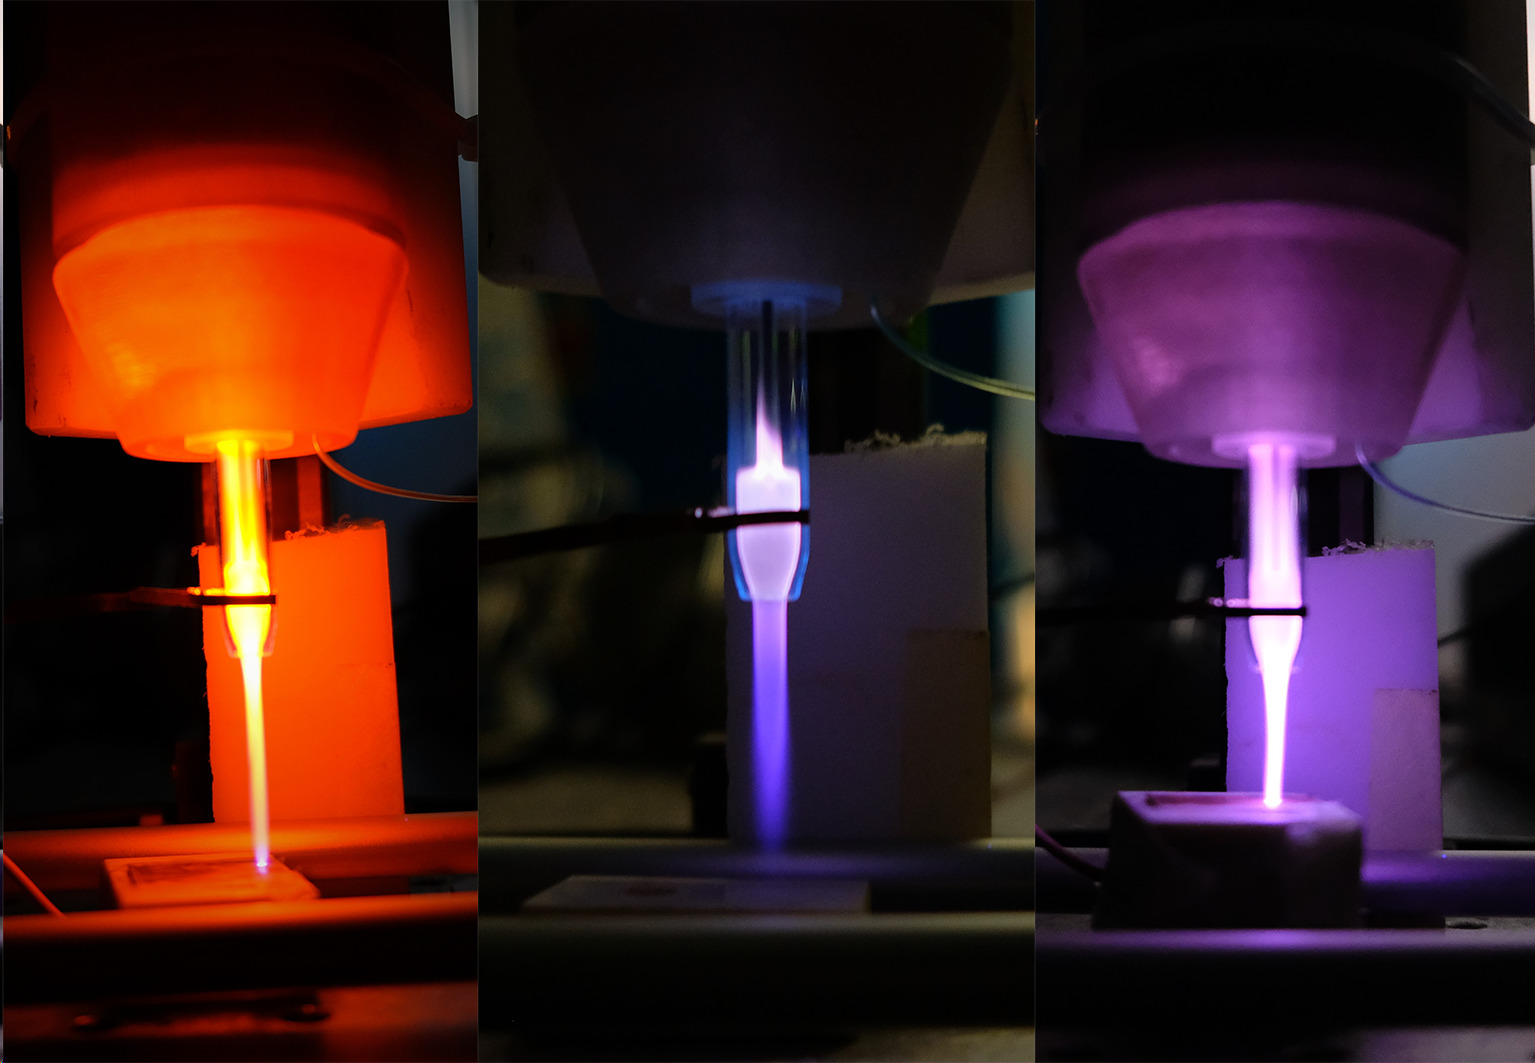
\includegraphics[width = 0.6\textwidth]{Images/Shape/plasmapic.png}
 \caption{Plasma plume pictures with different gasses used to start the discharge: neon on the left, argon in center and helium on the right. The source points to a conductive target positioned in front of the nozzle, after \SI{22}{\milli\meter} for neon and argon, after \SI{14}{\milli\meter} for helium.}
 \label{fig:pl_picture}
\end{figure}
\begin{figure}
 \centering
 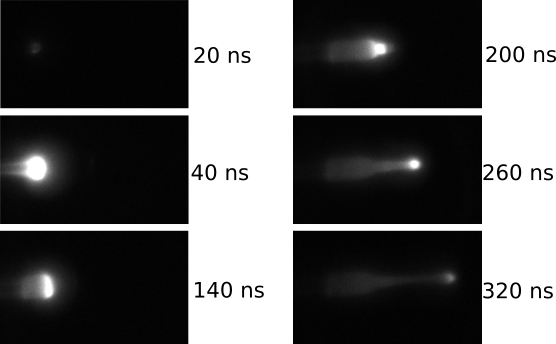
\includegraphics[width=0.8\textwidth]{Images/Shape/frames.png}
 \caption{Example of helium plasma bullet expulsion, as measured with our experimental setup. The single frames are taken with a fast camera with integration time of \SI{15}{\micro\second}.}
 \label{fig:pl_bullet}
\end{figure}

Plasma bullets still needs to be studied in depth, at today are known the basic dynamic of formation and expulsion. Some general features are that:
\begin{itemize}
 \item bullets velocities are $> \SI{10}{\kilo\meter/\second}$;
 \item bullet formation, it's velocity and it's travel distance depend on applied voltage on the electrode.
\end{itemize}

The scope of this experiment is to observe plasma bullets produced by our source, their shape and their velocity and how they change with different discharge conditions.

Given their typical velocities and the temperature of the plasma, bullet propagation is tought to be related to a travelling ionization front. This propagation can be studied with simplified simulation of DBD discharges, where it's reproduced the behaviour of plasma bullets (\cite{doi:10.1063/1.4963115}, \cite{Breden_2012}) or the interaction between plasma and a target (\cite{doi:10.1063/1.4923345}). Possible explanation for bullet propagation are analyzed at the end of this chapter, with estimation of electron temperature and mobility that give better insight on the phenomenology.
%We present a simple 1D model that can reproduce the propagation of this ionization front.

\section{Experimental setup}
To visually observe dynamics of plasma formation and propagation with enough resolution, it is needed an acquisition setup with a fast camera that has short integration time, below \SI{20}{\nano\second}, and an image intensifier that allows to visualize light emitted in such a short time interval.

To guarantee synchrony between plasma discharge and frame acquisition it is necessary to consider instruments and plasma source specific delays and give appropriate triggers.

Experimental setup is shown in photo \ref{fig:fotosetup} and a scheme is presented in \ref{fig:schemashape}. In the scheme there are the voltage signal lines that trigger the discharge and the acquisition, the optical acquisition apparatus pointed at source exit and the measurements acquisition instruments that are a computer and an oscilloscope. 
\begin{figure}
 \centering
 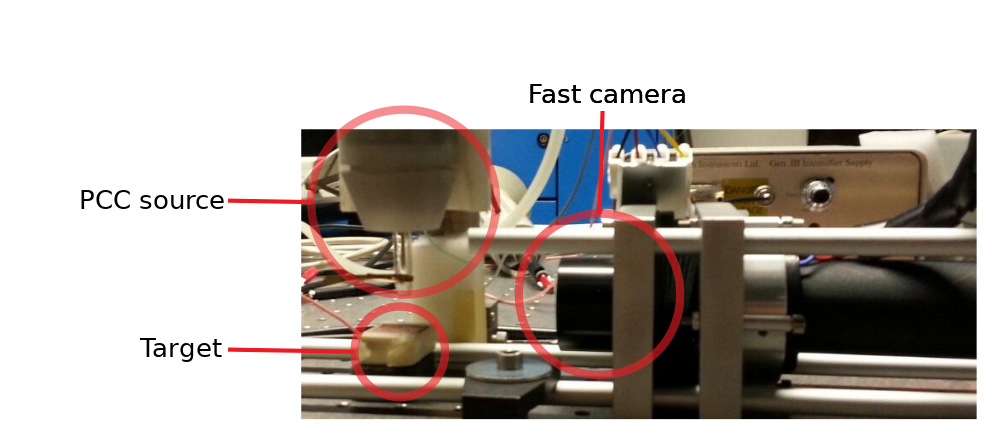
\includegraphics[width=0.8\textwidth]{Images/Shape/app_pic.png}
 \caption{Picture of the experimental setup. The source PCC is mounted vertically and points to a removable target that can be positioned at different heights. Plasma is observed with a fast camera from the side.}
 \label{fig:fotosetup}
\end{figure}
\begin{figure}
 \centering
 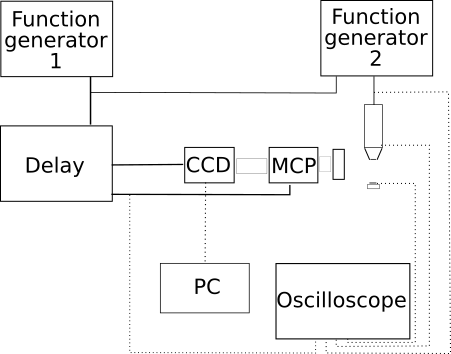
\includegraphics[width=0.5\textwidth]{Images/Shape/acq_ottica.png}
 \caption{Experimental setup scheme. Function generator 1, function generator 2 and delay generator send trigger signal to camera (CCD), to source and to image intensifier (MCP), full lines in the scheme. Camera sends measured frames to a computer (PC). From source, source's target, function generator 2 and delay are taken signals read on the oscilloscope, pointed lines in the scheme.}
 \label{fig:schemashape}
\end{figure}

\subsection{Source and optical setup}
Optical apparatus is composed by a lens %specific
 coupled with a Micro Channel Plate image intensifier (MCP). An MCP works as in figure \ref{fig:MCP}: for every photon received it emits many photons with little angular deviation.
\begin{figure}
 \centering
 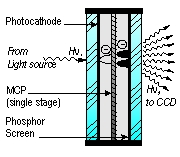
\includegraphics[width=0.4\textwidth]{Images/Shape/MCPsingle-stage.jpg}
 \caption{Micro Channel Plate image intensifier functioning.}
 \label{fig:MCP}
\end{figure}

Those photons are received by an high-speed camera \emph{Point Grey Flea} (\cite{flea}) equipped with a CCD of $\num{1024} \times \num{768}$ square pixels $\SI{4.75}{\micro\meter}$ wide. Every frame is sent to the pc where FLIR software elaborates and saves them in pgm format (\cite{pgm}).

\subsection{Source, power lines and electric signals}
The source utilized is the latest prototype, \textbf{B} in chapter \ref{ch:electric}. It has a voltage pulse peak value between $\num{3}$ and \SI{10}{\kilo\volt}, regulated by the lenght of the trigger signal $\Delta t$ (see chapter \ref{ch:electric}). To synchronyze measures and discharge the trigger signal a generator function gives the trigger signal (generator $2$ in the scheme) instead of the usual controller module of the source.

The source is positioned vertically at a distance of \SI{42.0(1)}{\milli\meter} from optical bench, with the glass nozzle that allows to observe plasma formation inside it (external diameter \SI{8.0(1)}{\milli\meter}, internal diameter \SI{6.0(1)}{\milli\meter}). The distance from the end of the electrode and nozzle exit is \SI{12}{\milli\meter}. At the exit the nozzle shrinks for \SI{3.0(1)}{\milli\meter}, until a diameter of \SI{5.0(1)}{\milli\meter}

Under the source is possible to position targets. Two different targets are used at different heights: a conductive target and an insulating target. The first one is a copper square sheet of dimensions $\SI{10}{\milli\meter} \times \SI{10}{\milli\meter} \times \SI{1}{\milli\meter}$ (used for current measures in chapter \ref{ch:electric}), the second one is a plastic material.

CCD camera is powered by a common voltage supply, while image intensifier MCP is powered by an high voltage supply. A delay generator trigger both instruments, with different delay times (see next section).

The oscilloscope \emph{Yokogawa DL9040}, utilized in chapter \ref{ch:electric}, reads on different channels the trigger signal given to source head, the trigger signal given to MPC, the voltage electrode with high-voltage probe \emph{Tektronix P6015A} and the current intensity when it's used the conductive target. Measurements of current intensity are done by a voltage probe with attenuation $\times \num{10}$ that measures the voltage drop on a resistance of $\SI{1}{\mega\ohm}$ connected to the conductive target.

\subsection{Trigger synchronization}
Experiment's objective is to observe plasma formation and propagation in synchronization with the measurement of voltage on the electrode, so it's necessary to know precisely discharge and measure times.

The trigger lines is composed with:
\begin{itemize}
 \item function generator \emph{Or-x 310}, $1$ in figure, that sends a square pulse with set amplitude and width, with pulse repetition rate $f$;
 \item function generator \emph{Lecroy 9210}, $2$ in figure, that sends a square wave with repetition rate given by the trigger, with constant amplitude and variable width $\Delta t$;
 \item delay time generator \emph{Stanford DG535}, that sends a square wave with constant amplitude and repetition rate given by the voltage input. Start time of this signal is given by input starting time plus settable delays (4 different channels).
\end{itemize}

Every measuring instrument has it's own time delay between trigger signal and effective measure. The higher delay is the arming time for fast camera, in the order of \si{\milli\second}, the shortest one is the integration time for acquisition system, that starts from the activation of the image intensifier and span $\SI{15}{\nano\second}$.

A time line is shown in figure \ref{fig:times}, an example of signals taken with the oscilloscope is in figure \ref{fig:times_signals}. There are three relevant times defined by function and delay generators:
\begin{enumerate}
 \item $t_{0}$ is the starting time for the square pulse given by \emph{Function generator 1}, with an amplitude of $\SI{5}{\volt}$ and repetition rate $f$. The pulse is the external trigger for \emph{Function generator 2} and the voltage input of \emph{Delay generator}. The square wave that triggers the voltage pulse on the source starts at $t_{0}$ from \emph{Function generator 2}; it has a time width of $\Delta t$ that defins voltage amplitude (see chapter \ref{ch:electric}) and repetition rate $f$. The trigger signal that arms the camera starts at $t_{0}$ from \emph{Delay generator}.
 \item $t_{\text{DIS}}$ is the effective discharge starting time, when the voltage peak starts. From trigger signal end to voltage peak start there is a time delay given mainly by the response time of the photodiode on source head. Measuring the signals as in figure \ref{fig:times_signals}, it's possible to estimate this delay as $\SI{987.7(567)}{\nano\second}$, constant for every $f$ and $\Delta t$. The discharge happens after $t_{\text{DIS}}$, measurement times must be inside the grey zone in the scheme.
 \item $t_{\text{MIS}}$ is the measurement time, when MCP is triggered on. \emph{Delay generator} gives the delay between $t_{0}$ and $t_{\text{MIS}}$, called $t_{D}$, with possible steps of \SI{1}{\pico\second}. Changing $t_{D}$ it's possible to see plasma dynamics at different times that corresponds to different electrode voltage values, as in figure \ref{fig:times_signals}.
\end{enumerate}
\begin{figure}
 \centering
 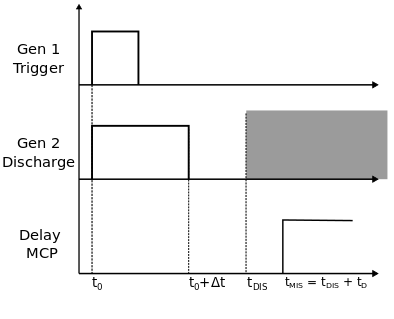
\includegraphics[width=0.6\textwidth]{Images/Shape/times.png}
 \caption{Time signal synchronization scheme: $t_{0}$ is the starting trigger time, $\Delta t$ is the opening time for plasma source (see chapter \ref{ch:electric}), $t_{\text{DIS}}$ is the starting time for the discharge and $t_{\text{MIS}}$ the starting time for the MCP i.e. the measure time}.
 \label{fig:times}
\end{figure}
\begin{figure}
 \centering
 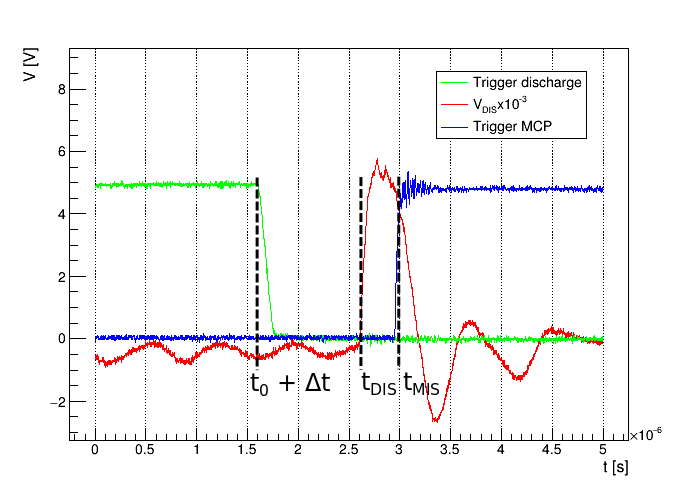
\includegraphics[width=0.6\textwidth]{Images/Shape/times_osc_2.png}
 \caption{Example of oscilloscope measure. In green the discharge trigger, in red the electrode voltage output and in blue the MCP trigger. The dashed lines indicate times described in \ref{fig:times}.}
 \label{fig:times_signals}
\end{figure}


Integration time for a single frame is \SI{15}{\nano\second}, so the time step between two measures has to be larger then it. Time steps chosen are \SI{20}{\nano\second} for high resolution mesurements, \SI{50}{\nano\second} for standard measurements.

It's important to point out that pulse repetition rates are $f \ge \SI{1}{\kilo\hertz}$ corresponding to a time interval between two pulses lower then \SI{1}{\milli\second}; while the measure interval time between the acquisition of two frames is larger then \SI{50}{\milli\second} beacause of the camera. It is not possible to see two consecutive times for the same discharge, the frames are always measures of different discharges.

Eaxh pixel on the CCD has a minimum and maximum intensity value, is possible to mantain the measure on the wanted level changing the settings on camera acquisition software.
One of the parameters is the \emph{Shutter time}, the opening time of the camera shutter. If the emission intensity is too low we can set the shutter time larger then the time between two acquisition, to acquire a frame that is the sum of two discharge.
Another parameter is the \emph{Gain} value, that amplifies or reduces the output.
For each used gas we select an appropriate \emph{Gain} value and an appropriate \emph{Shutter time}.

\subsection{Different setups}
Many parameters have an effect on plasma formation: voltage pulse repetition rate, voltage rise time, voltage peak value, gas type, gas flow, presence of a target and its features (see \cite{Mericam_Bourdet_2009}, \cite{Jarrige_2010}).
This study presents different setups with three different gasses, as shown in table \ref{tab:setups}.
There is a lower limit value for pulse repetition rate, different for each gas, under which there is no discharge. The electric behavior of the source is the same for values higher than this threshold (see chapter \ref{ch:electric}). For each gas is chosen a repetition rate value that allows the discharge to start.

Gasses with different composition will have different ionization reactions and will produce different reactive species, with different masses and ionization energies. With this study is possible to observe how peak voltage value, gas type and gas flow determine plasma bullet formation and affect its expulsion velocity.

A conductive target near plasma exit at ground potential will modify the electric field produced by the electrode. With this study is possible to observe how the target affects bullet expulsion and propagation. Furthermore the bullet can hit the target, introducing into reactions balance also the electrons on the target.

When argon is the neutral gas used to start the discharge a grounded conductive ring can be placed around the nozzle after the electrode, to help the start of the discharge.
\begin{table}
 \centering
 \begin{tabular}{cccccccc}
  \toprule
  Gas   &Setup  &$\Delta t$ [\si{\micro\second}] &Target &Target position [\si{\milli\meter}] &Flow rate [\si{\liter/\minute}]  &Other  &$\Delta t_D$ [\si{\nano\second}]\\
  \midrule
  \multirow{7}*{\ce{He}}    &A  &\num{3}, \num{3.5}, \num{4} &-  &-  &\num{2} &-  &\num{20}\\
                            &B  &\num{3.5} &-  &-  &\num{1}  &-  &\num{20}\\
                            &C  &\num{3.5} &-  &-  &\num{3}  &-  &\num{20}\\
                            &D  &\num{3.5} &-  &-  &\num{4}  &-  &\num{20}\\
                            &E  &\num{3}, \num{3.5}, \num{4} &Insulator  &\num{24}  &\num{2} &-  &\num{20}\\
                            &F  &\num{3}, \num{3.5}, \num{4} &Conductor  &\num{32}  &\num{2} &-  &\num{20}\\
                            &G  &\num{3}, \num{3.5}, \num{4} &Conductor  &\num{24}  &\num{2} &-  &\num{20}\\
  \midrule
  \multirow{4}*{\ce{Ne}}    &A  &\num{2}, \num{2.5}, \num{3} &Insulator  &\num{24}  &\num{2} &-  &\num{50}\\
                            &B  &\num{2}, \num{2.5}, \num{3} &Conductor  &\num{32}  &\num{2} &-  &\num{50}\\
                            &C  &\num{2}, \num{2.5}, \num{3} &Conductor  &\num{24}  &\num{2} &-  &\num{50}\\
                            &D  &\num{2}, \num{2.5}, \num{3} &-  &-  &\num{2} &-  &\num{50}\\
  \midrule
  \multirow{6}*{\ce{Ar}}    &A  &\num{3.5} &-  &-  &\num{2} &Grounded ring  &\num{50}\\
                            &B  &\num{3.5} &-  &-  &\num{2} &-  &\num{50}\\
                            &C  &\num{3.5} &Conductor  &\num{20}  &\num{2} &Grounded ring  &\num{50}\\
                            &D  &\num{3.5} &Conductor  &\num{20}  &\num{2} &-  &\num{50}\\
  \bottomrule
 \end{tabular}
 \caption{Description of measure setups. In first column there is the gas; second column is the setup name; third column is voltage pulse time width; four and fifth columns are target information, if it's used a target; sixth column is gas flow; seventh column are other informations, e.g. if it's positioned a grounded ring around the nozzle; eight column is the time step between acquisitions.}
 \label{tab:setups}
\end{table}

\begin{comment}
\begin{table}
 \centering
 \begin{tabular}{cccccccc}
  \toprule
  Gas   &Setup  &$\Delta t$ [\si{\micro\second}] &Target &Target position    &Flow rate  &Other  &$\Delta t_D$ [\si{\nano\second}]\\
  \midrule
  \multirow{8}*{\ce{He}}    &A  &$\num{30}, \num{35}, \num{40}$ &Conductor  &\SI{24}{\milli\meter}  &\SI{2}{\liter/\minute} &-  &\SI{50}{\nano\second}\\
                            &B  &$\num{30}, \num{35}, \num{40}$ &Conductor  &\SI{32}{\milli\meter}  &\SI{2}{\liter/\minute} &-  &\SI{20}{\nano\second}\\
                            &C  &$\num{30}, \num{35}, \num{40}$ &Insulator  &\SI{24}{\milli\meter}  &\SI{2}{\liter/\minute} &-  &\SI{20}{\nano\second}\\
                            &D  &$\num{30}, \num{35}, \num{40}$ &-  &-  &\SI{2}{\liter/\minute} &-  &\SI{20}{\nano\second}\\
                            &E  &$\num{35}$ &-  &-  &\SI{2}{\liter/\minute} &Ground ring  &\SI{20}{\nano\second}\\
                            &F  &$\num{35}$ &-  &-  &\SI{1}{\liter/\minute} &-  &\SI{20}{\nano\second}\\
                            &G  &$\num{35}$ &-  &-  &\SI{3}{\liter/\minute} &-  &\SI{20}{\nano\second}\\
                            &H  &$\num{35}$ &-  &-  &\SI{4}{\liter/\minute} &-  &\SI{20}{\nano\second}\\
  \midrule
  \multirow{5}*{\ce{Ne}}    &A  &$\num{20}, \num{25}, \num{30}$ &Conductor  &\SI{24}{\milli\meter}  &\SI{2}{\liter/\minute} &-  &\SI{50}{\nano\second}\\
                            &B  &$\num{20}, \num{25}, \num{30}$ &Conductor  &\SI{32}{\milli\meter}  &\SI{2}{\liter/\minute} &-  &\SI{50}{\nano\second}\\
                            &C  &$\num{20}, \num{25}, \num{30}$ &Insulator  &\SI{24}{\milli\meter}  &\SI{2}{\liter/\minute} &-  &\SI{50}{\nano\second}\\
                            &D  &$\num{20}, \num{25}, \num{30}$ &-  &-  &\SI{2}{\liter/\minute} &-  &\SI{50}{\nano\second}\\
                            &E  &$\num{30}$ &-  &-  &\SI{2}{\liter/\minute} &Ground ring  &\SI{50}{\nano\second}\\
  \midrule
  \multirow{6}*{\ce{Ar}}    &A  &$\num{35}$ &-  &-  &\SI{2}{\liter/\minute} &Ground ring  &\SI{50}{\nano\second}\\
                            &B  &$\num{35}$ &-  &\SI{32}{\milli\meter}  &\SI{2}{\liter/\minute} &-  &\SI{20}{\nano\second}\\
                            &C  &$\num{35}$ &-  &-  &\SI{2}{\liter/\minute} &Floating ring  &\SI{50}{\nano\second}\\
                            &D  &$\num{35}$ &Conductor  &\SI{20}{\milli\meter}  &\SI{2}{\liter/\minute} &Ground ring  &\SI{50}{\nano\second}\\
                            &E  &$\num{35}$ &Conductor  &\SI{20}{\milli\meter}  &\SI{2}{\liter/\minute} &-  &\SI{50}{\nano\second}\\
                            &F  &$\num{35}$ &-  &-  &\SI{2}{\liter/\minute} &-  &\SI{50}{\nano\second}\\
                            &G  &$\num{35}$ &Conductor  &\SI{32}{\milli\meter}  &\SI{2}{\liter/\minute} &-  &\SI{50}{\nano\second}\\
  \bottomrule
 \end{tabular}
 \caption{Description of measure setups. In first column there is the gas; second column is the setup name; third column is voltage pulse time width, expressed as percentage of a square trigger \SI{10}{\micro\second} long; four and fifth columns are target information, where it's used a target; sixth column is used gas flow; seventh column are other informations, i.e. if it's used the conductor ring explained before; eight column is the time step between two different frames.}
 \label{tab:setups}
\end{table}
\end{comment}

\subsection{Frame analysis and calibration}
Once a measure setup is chosen, the first acquisition is set around the start of the discharge. On the oscilloscope is saved the signal waveform for every channel (setup as explained before), on the computer $5$ frames for every $t_D$ are saved. Measures are taken with steps of $\Delta t_D$ until it is not possible to observe plasma anymore.

Measure time from the start of the discharge can be evaluated from waveforms on the oscilloscope.

Frame analysis is done converting the pgm files in 2-dimensional histograms, with \emph{TH2} class written in \emph{ROOT} libraries (see \cite{ROOT:TH2}).
%We are interested in plasma bullet formation and it's expulsion, but also in other fenomenological behaviour that is observed during measures.

From the five frames taken it is evaluated the average value for each pixel. From the resulting frame the plasma bullet is isolated as the collection of pixels with maximum intensity in the frame. The estimation of the bullet position is given by the coordinates of its luminosity barycenter on the plane seen by camera, called x-y in the analysis.
Once established the center, the points were luminosity goes under a certain percentage of the maximum define its contour. Bullet dimensions along x and y axis are evaluated from the contour, while average luminosity is given by pixel values inside the contour.
With barycenter coordinates it's possible to compute bullet velocity using a finite difference formula \cite{Bhadauria}.


Frame dimensions are found through a calibration with a known target: at plasma exit is positioned a plate with $4$ holes, diameter of \SI{1.0(1)}{\milli\meter} at the vertices of a square with an edge lenght of \SI{10.0(1)}{\milli\meter}, and illuminated from behind with a torch.
For the frame of this setup it's possible to extrapolate the pixel distance that corresponds to \SI{10}{\milli\meter} for every square edge, average them, and calculate pixel's width in frames, resulting a value of $d_{pix} = \SI{0.172(2)}{\milli\meter}$.


\section{Helium flow}
Helium it's an element with standard atomic weight of $\num{4.002}$, 1st ionization energy of \SI{24.587}{\electronvolt} and 2nd ionization energy of \SI{54.418}{\electronvolt}.
It is easy to produce helium plasma, when ionized it emits radiation with principal wavelengths in violet and orange ($\lambda = \num{388.86}$ and \SI{587.56}{\nano\meter}).

In this work helium plasma is produced with pulse repetition rate $f = \SI{5}{\kilo\hertz}$ and different voltage peak values, as explained in table \ref{tab:setups}.
Delays are setted to take a single frame during every acquisition, for every measure are acquired $5$ frames.

\subsection{Plasma bullet description}
A description of bullet propagation can be given with setup A, for $\Delta t = \SI{3.5}{\micro\second}$, i.e. absence of a target and gas flow of \SI{2}{\liter/\minute}.

It's possible to divide the phenomenon in four phases, as presented in figure \ref{fig:bullet_es}: bullet formation, bullet displacement inside the nozzle, bullet expulsion and bullet propagation outside the nozzle, in air. %It's important to remember that time values goes from the start of the voltage peak, extrapolated from oscilloscope measures.
When the voltage goes over a definite value, a rapid increase in luminosity is observed around the electrode. From there, in a time of $\sim \SI{50}{\nano\second}$ the plasma modifies it'shape and becames the bullet: a zone with high luminosity confined in space. The bullet then moves in the exit direction and it's expelled always with a well defined front. The round shaped bullet propagation can be seen in air until it reaches a maximum travel distance and then luminosity decreases rapidly. In these measurements conditions plasma forms again in correspondence of the negative tension peak, but it is a rapid process without propagation.
\begin{figure}
 \centering
 \subfloat[\SI{140.93}{\nano\second}]{
    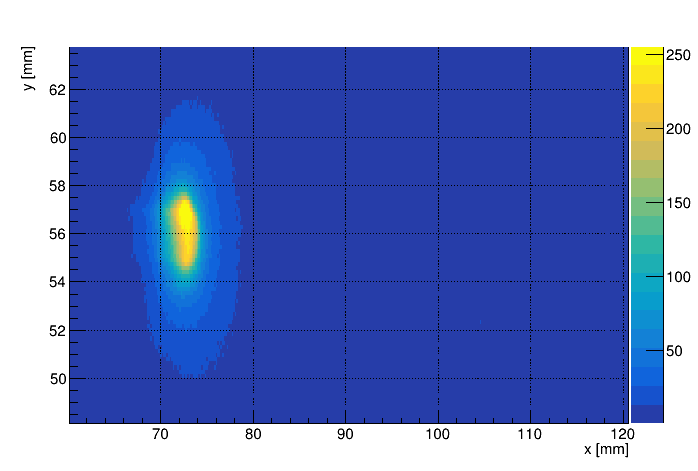
\includegraphics[width=0.48\textwidth]{Images/Shape/elio_d035_es1.png}
 }
 \hfill
 \subfloat[\SI{240.93}{\nano\second}]{
    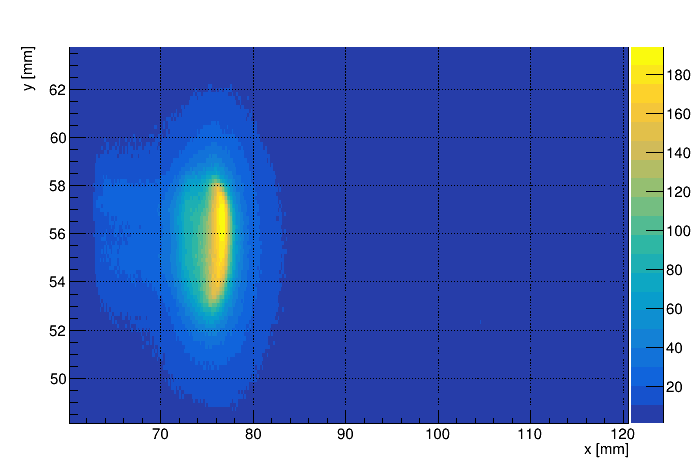
\includegraphics[width=0.48\textwidth]{Images/Shape/elio_d035_es2.png}
 }
 
 \subfloat[\SI{400.93}{\nano\second}]{
    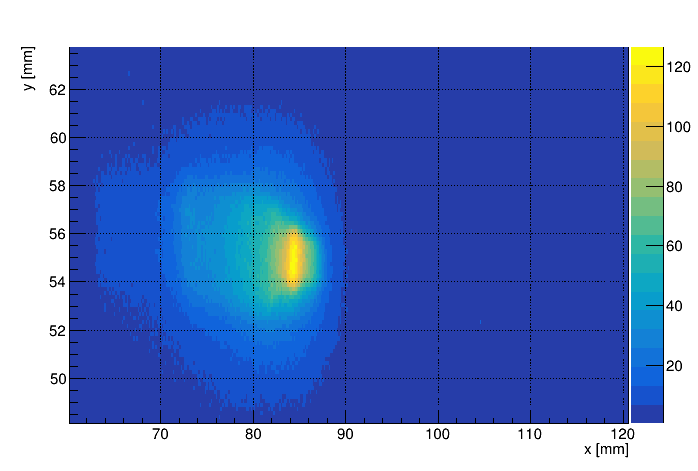
\includegraphics[width=0.48\textwidth]{Images/Shape/elio_d035_es3.png}
 }
 \hfill
 \subfloat[\SI{460.93}{\nano\second}]{
    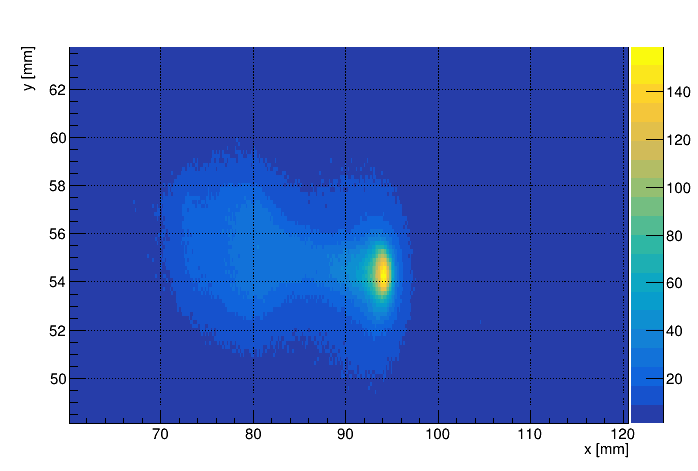
\includegraphics[width=0.48\textwidth]{Images/Shape/elio_d035_es4.png}
 }
 \caption{Four phases of plasma dynamics: bullet formation (a), bullet displacement inside the nozzle (b), bullet expulsion (c) and bullet propagation outside the nozzle (d). Time intervals are calculated from the start of the voltage peak.}
 \label{fig:bullet_es}
\end{figure}


\paragraph{Electrode voltage and bullet intensity}
The time interval where there is the bullet can be defined as where it is possible to see a definite zone with mean luminosity higher then the background. The starting time is given by voltage reaching a certain value, and the bullet expires when it's luminosity decreases.

The average intensity value inside the bullet and the voltage measurement in the intersted time interval are presented in figure \ref{fig:elio_d035_I}. Plasma formation is observed around \SI{120.93}{\nano\second} after peak start, at a tension value of \SI{5710.00(28550)}{\volt}. %while maximum peak value is \SI{6588.80(32944)}{\volt} at time \SI{260.93}{\nano\second}.
Luminosity is higher during plasma formation around the electrode and it decrease very little during all the propagation, even after the expulsion in air (pointed line on the graph). After a time of \SI{440}{\nano\second} the bullet luminosity decreases rapidly and it disperses in the air.
\begin{figure}
 \centering
 \subfloat[Zoom on voltage waveform.]{
    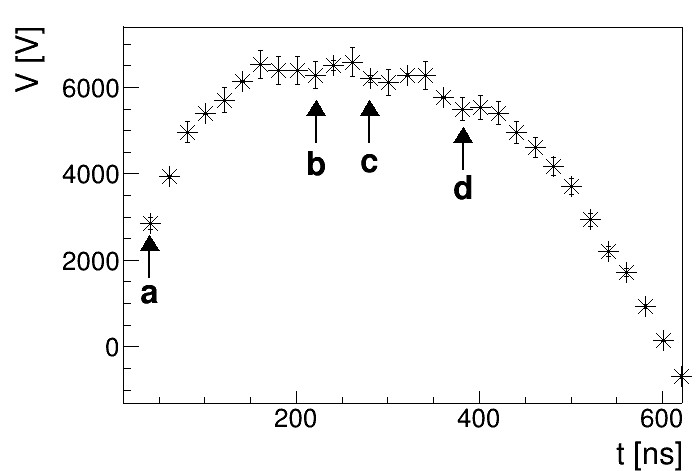
\includegraphics[width=0.48\textwidth]{Images/Shape/elio_d035_V.png}
 }
 \hfill
 \subfloat[Mean intensity of plasma bullet.]{
    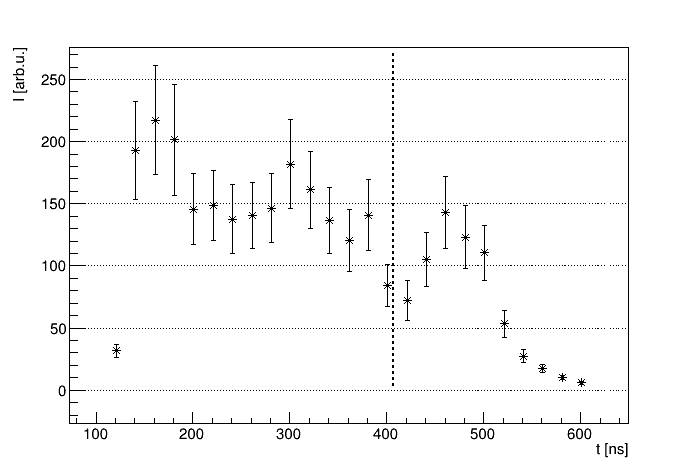
\includegraphics[width=0.48\textwidth]{Images/Shape/elio_d035_Im.png}
 }
 \caption{Voltage waveform and intensity of the bullet versus time, measurements setup A with voltage peak of \SI{6.6}{\kilo\volt}. Time zero is the start of the voltage peak, ending time is taken as the time where intensity reaches background value. The dashed line for intensity indicates when the bullet reaches the end of the nozzle.}
 \label{fig:elio_d035_I}
\end{figure}

\paragraph{Barycenter coordinates and direction}
The motion of the bullet on observing plane can be extrapolated from its barycenter coordinates.

In figure \ref{fig:elio_d035_bary} there are the two coordinates for different times.
Coordinate x, along the axis of the source is more relevant to observe bullet expulsion. Plasma forms around position $\SI{73}{\milli\meter}$ and the nozzle ends at $\SI{85}{\milli\meter}$, compatible with the distance described before. Plasma bullet moves in the nozzle with a certain velocity, until it reaches the exit and propagates in the air more rapidly. In air the bullet travels until it reaches a maximum x, covering a distance of \SI{26.08(2)}{\milli\meter} from the electrode. The bullet stops before its luminosity reaches the minimum value.

Coordinate y it's relevant to show bullet direction. From figure it is possible to see that  it moves in a space interval of \SI{2}{\milli\meter}. The bullet forms over the electrode, then it enlarges to cover all the nozzle diameter and lowers it's barycenter with a constant slope, even after the expulsion. Once the bullet starts to decrease in luminosity, it stops its motion also on the y direction.
\begin{figure}
 \centering
 \subfloat[]{
    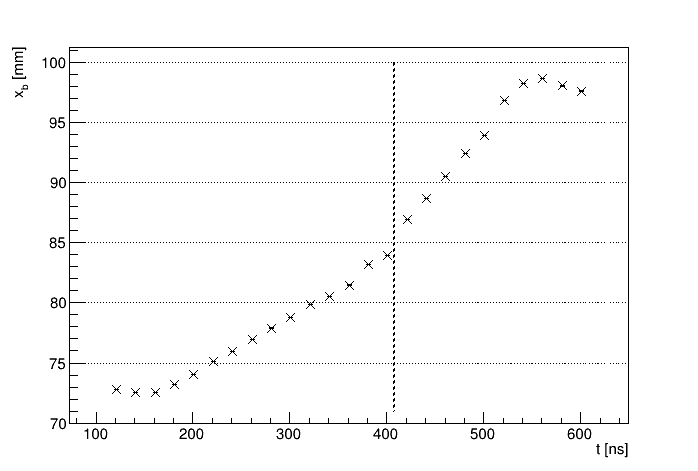
\includegraphics[width=0.48\textwidth]{Images/Shape/elio_d035_xb.png}
 }
 \hfill
 \subfloat[]{
    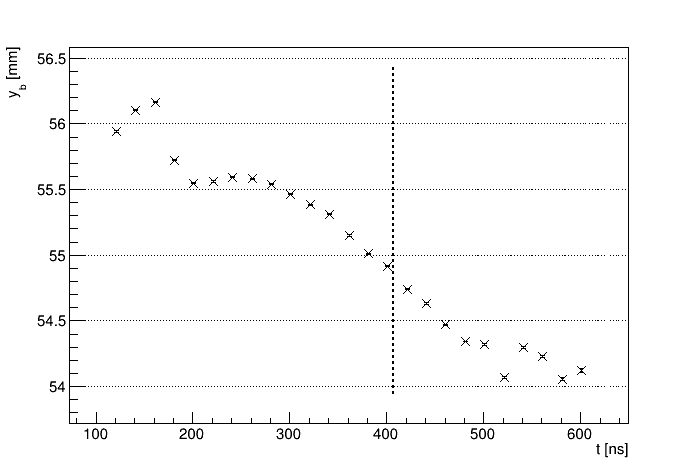
\includegraphics[width=0.48\textwidth]{Images/Shape/elio_d035_yb.png}
 }
 \caption{Barycenter coordinates of the bullet for measurements setup A with voltage peak of \SI{6.6}{\kilo\volt}. Pointed lines indicate the end of the nozzle.}
 \label{fig:elio_d035_I}
\end{figure}

Baricenter motion in the y direction it's explainable by a tilt in the source, that is not perfectly perpendicular to the optical bench. In figure \ref{fig:elio_d035_diry} there is the countour of the bullet in the y direction in function of the x brycenter coordinate, is possible to see that the figure is inclined. Inside the nozzle y maximum is the value that defines the contour of the nozzle, the angle of inclination is given by a linear fit as in figure and it is \SI{3.39(10)}{\degree}. Outside the nozzle the barycenter direction is inclined at an angle of \SI{3.71(4)}{\degree}. The values are almost compatible with each other, so it seems that tilting the source it is possible to direct the bullet even after its propagation in air.
\begin{figure}
 \centering
 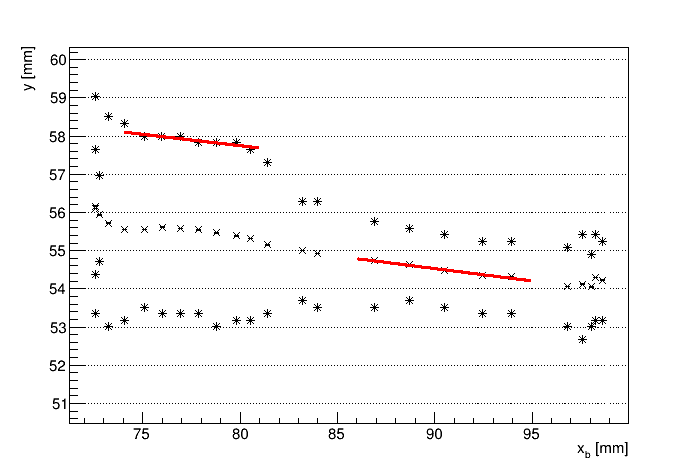
\includegraphics[width=0.6\textwidth]{Images/Shape/elio_d035_incl.png}
 \caption{Countour of the bullet in y direction as a function of barycenter coordinate x, for measurements setup A with voltage peak of \SI{6.6}{\kilo\volt}. For each x value is possible to see y maximum, y minimum and y barycenter of the bullet. There are two linear fits to compare the inclination of the source (first linear fit of y maximum inside the nozzle) with the inclination of bullet propagation direction in air (second linear fit of y barycenter).}
\end{figure}


\paragraph{Bullet dimensions}
Once the contour of the bullet is defined, it is simple to evaluate its dimensions along x and y directions, in figure \ref{fig:elio_d035_dim} are presented the results for each time.
.
In the x direction, the bullet presents constant diameter until it approaches nozzle exit, where it enlarges to reach the exit. In air the bullet mantaines its dimension, with lower values then inside the nozzle, but compatible within the error. When it stops the measure loses significance as the bullet loses luminosity and it is not distinguishable from the background.
In y direction there is a constant value of \SI{4.65(20)}{\milli\meter} during propagation in the nozzle, as expected because the bullet covers all the nozzle area. Once the nozzle shrinks, the bullet diminish it's diameter and maintains a constant value of \SI{2.07(20)}{\milli\meter} during all the propagation in air.
\begin{figure}
 \centering
 \subfloat[]{
    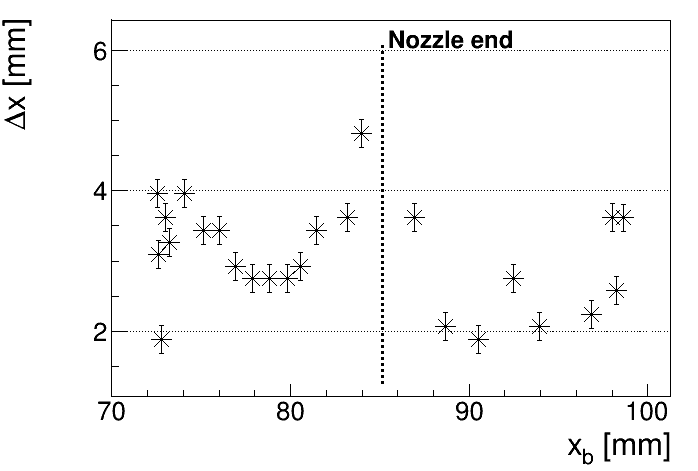
\includegraphics[width=0.48\textwidth]{Images/Shape/elio_d035_dx.png}
 }
 \hfill
 \subfloat[]{
    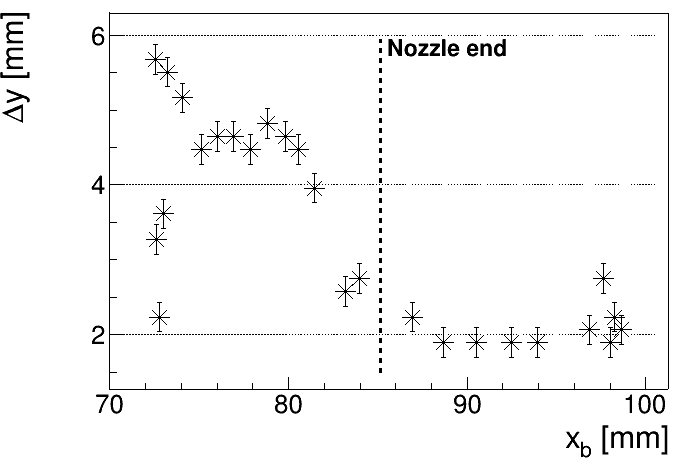
\includegraphics[width=0.48\textwidth]{Images/Shape/elio_d035_dy.png}
 }
 \caption{Dimensions of the bullet for measurements setup A with voltage peak of \SI{6.6}{\kilo\volt}. Pointed lines indicate the end of the nozzle.}
 \label{fig:elio_d035_I}
\end{figure}


\paragraph{Bullet velocity}
From barycenter graphs it is possible to estimate the bullet velocity at different times.
With a linear fit of the x barycenter inside the nozzle, as shown in figure \ref{fig:elio_d035_vx}, bullet velocity is found to be $v_{N} = \SI{46.48(20)}{\kilo\meter/\second}$. Once it exits the nozzle the speed goes up, until a value of $v_{A} = \SI{95.16(60)}{\kilo\meter/\second}$.

Velocity for each time can be calculated with a 3 point finite difference formula (that excludes the first and the last point), finding the values shown in figure \ref{fig:elio_d035_vx}. The average velocity value inside the nozzle and in air is compatible with the result from the linear fit: $v_{N} = \SI{48.23(103)}{\kilo\meter/\second}$ and $v_{A} = \SI{95.16(182)}{\kilo\meter/\second}$.
\begin{figure}
 \centering
 \subfloat[Fit of x barycenter.]{
    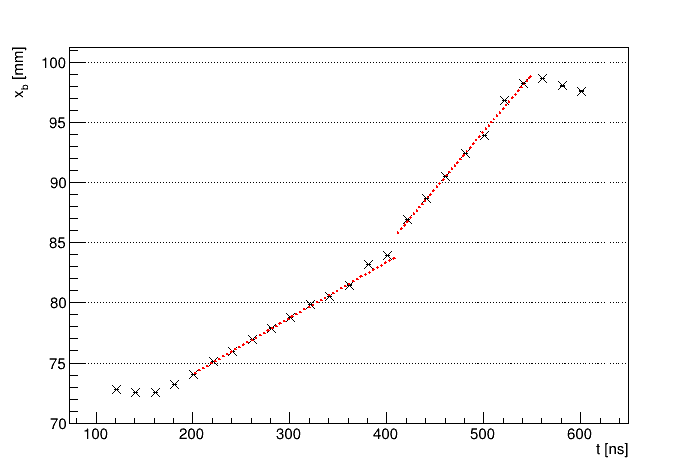
\includegraphics[width=0.48\textwidth]{Images/Shape/elio_d035_xb_fitv.png}
 }
 \hfill
 \subfloat[Velocities in x direction.]{
    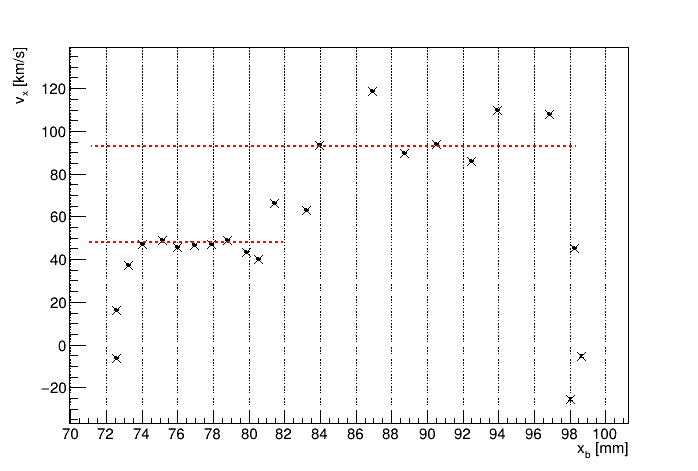
\includegraphics[width=0.48\textwidth]{Images/Shape/elio_d035_vx_fitv.png}
 }
 \caption{Velocity of the bullet in x direction for measurements setup A with voltage peak of \SI{6.6}{\kilo\volt}. In (a) linear fit of barycenter position as function of time inside the nozzle and in air; in (b) velocities evaluated for each time with a three point difference formula, where dashed lines indicate average values inside the nozzle and in air.}
 \label{fig:elio_d035_vx}
\end{figure}

It's interesting to point out that those velocities are much higher then the average velocity of the neutral gas: for a flow of \SI{2}{\liter/\minute} it is of \SI{12}{\meter\second}.


\subsection{Voltage influence}
An increase in trigger width $\Delta t$ correspond to an increase in voltage peak values (see chapter \ref{ch:electric}) and an increase in electric field intensity. The voltage peak value could change bullet formation and propagation. The results of the analysis for setup A with different voltage values are in figure \ref{fig:elio_d} and table \ref{tab:elio_d}.

The discharge starts always in the same voltage interval, around \SI{5.7}{\kilo\volt}. At an higher voltage corresponds an higher luminosity, but the time interval where luminosity decreases is always around \SI{100}{\nano\second} once it exits the nozzle (figure \ref{fig:elio_d} (a)).

The plot for the barycenter coordinates (figure \ref{fig:elio_d} (b) - (c)) shows that higher voltage corresponds to further distances reached by the bullet ($x_{\text{dist}}$ and $y_{\text{dist}}$ in table). For the lower voltage peak the bullet doesn't even propagate in air, as it stops right after nozzle exit.

Dimensions of the bullet (figure \ref{fig:elio_d} (d) - (e)) are not influenced by voltage value, they have the exact same behaviour for every measurements set. A single notable difference it's in the y diameter inside the nozzle, where for higher voltage there are slightly larger values. However inside the nozzle there are refraction effects due to the glass, the increase is compatible with the variation in dimensions that could be given by higher luminosity.

Velocity values (figure \ref{fig:elio_d} (f)) show how the bullet behaviour is costant during the propagation inside the nozzle and becames more erratic once it exits.
As mentioned before, for the lowest voltage value the bullet stops right after it exits the nozzle, in this configuration it's not possible to find a propagation velocity in air. For other sets velocity has the same profile, with a proportionality between peak voltage value and velocity value: increasing voltage velocity goes from $v_{A} = \SI{92.93(6)}{\kilo\meter/\second}$ to $v_{A} = \SI{149.47(9)}{\kilo\meter/\second}$.
\begin{figure}
 \centering
 \subfloat[Mean luminosity.]{
    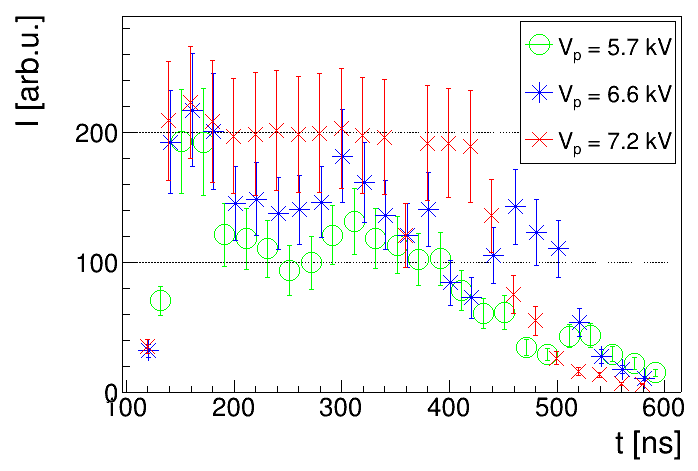
\includegraphics[width=0.48\textwidth]{Images/Shape/elio_d_Im.png}
 }
 \hfill
 \subfloat[x barycenter.]{
    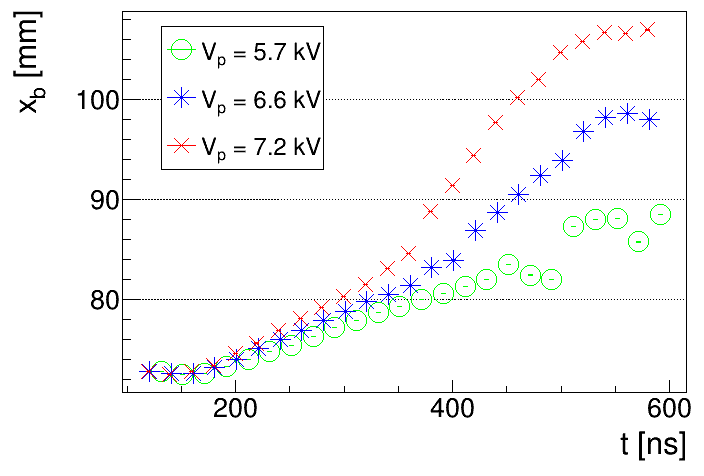
\includegraphics[width=0.48\textwidth]{Images/Shape/elio_d_xb.png}
 }
 \subfloat[y barycenter.]{
    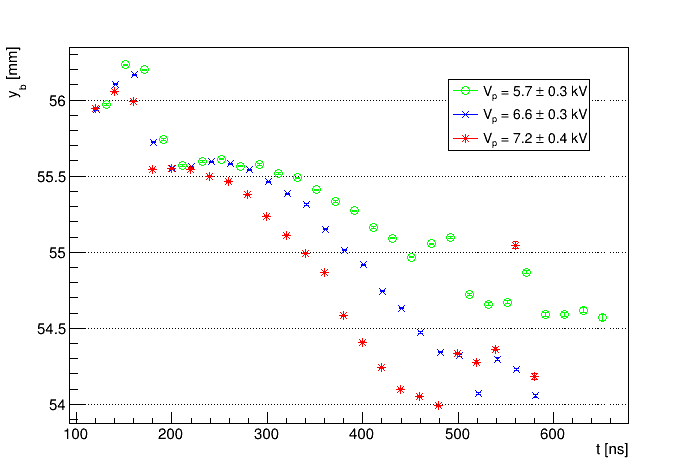
\includegraphics[width=0.48\textwidth]{Images/Shape/elio_d_yb.png}
 }
 \hfill
 \subfloat[x diameter.]{
    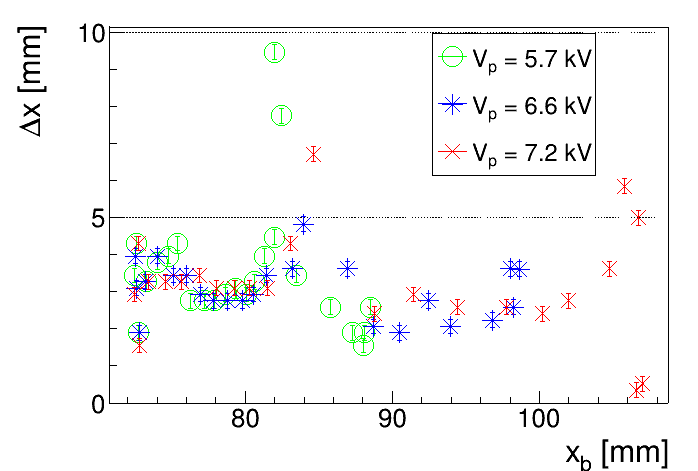
\includegraphics[width=0.48\textwidth]{Images/Shape/elio_d_dx.png}
 }
 \subfloat[y diameter.]{
    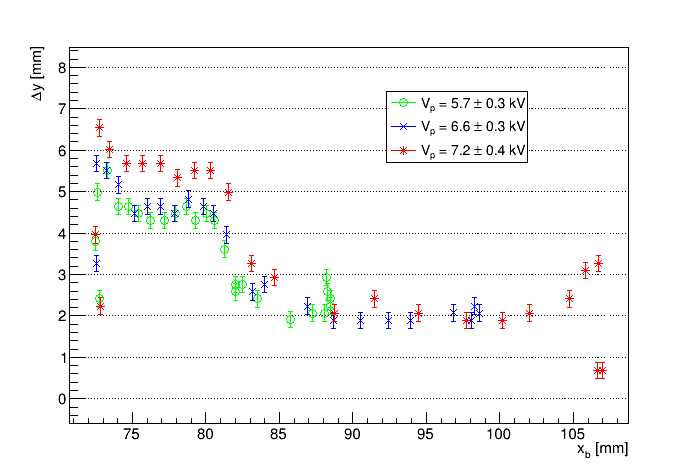
\includegraphics[width=0.48\textwidth]{Images/Shape/elio_d_dy.png}
 }
 \hfill
 \subfloat[x velocity.]{
    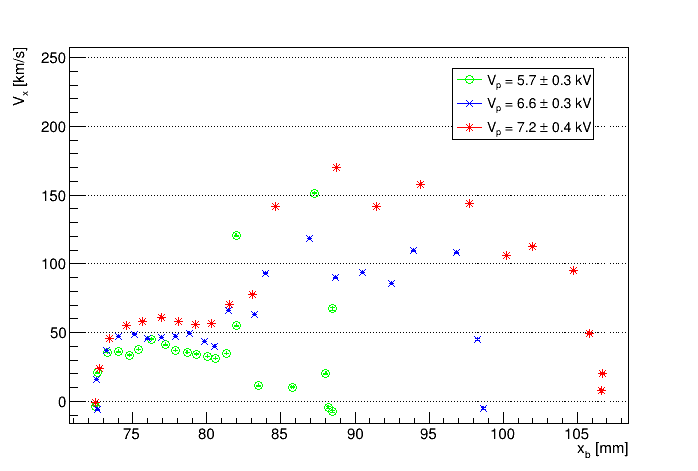
\includegraphics[width=0.48\textwidth]{Images/Shape/elio_d_vx.png}
 }
 \caption{Results of the analysis for setup A (helium flow of \SI{2}{\liter/\minute} without target), with different peak voltage values.}
 \label{fig:elio_d}
\end{figure}

\begin{comment}
\begin{table}
 \centering
 \begin{tabular}{ccccccc}
 \toprule
 $V_{p}$ [kV]    &$t_{0}$ [ns] &$V_{0}$ [kV]    &$x_{\text{dist}}$ [mm]   &$y_{\text{dist}}$ [mm]   &$v_{N}$ [km/s]   &$v_{A}$ [km/s]\\
 \midrule
 \num{5.66(30)}  &\num{131.5}  &\num{5.55(28)}    &\num{15.99(1)} &\num{1.66(2)}  &\num{37.72(4)} &-\\
 \num{6.59(33)}  &\num{120.9}  &\num{5.71(29)}    &\num{26.08(2)} &\num{1.92(4)}  &\num{46.48(2)} &\num{95.16(6)}\\
 \num{7.22(36)}  &\num{119.5}  &\num{6.01(30)}    &\num{34.55(5)} &\num{2.07(1)}  &\num{59.80(3)} &\num{149.47(9)}\\
 \bottomrule
 \end{tabular}
 \caption{Result of the analysis with different voltage peak values for the pulse. $V_{p}$ is the peak value for the pulse, $t_{0}$ bullet formation time, $V_{0}$ bullet formation tension, $x_{\text{dist}}$ and $y_{\text{dist}}$ are the highest distances reached by the bullet from electrode position, $v_{N}$ is the velocity in x direction reached inside the nozzle, $v_{A}$ is the velocity of propagation in air in x direction.}
 \label{tab:elio_d}
\end{table}
\end{comment}

\begin{table}
 \centering
 \begin{tabular}{cccccc}
 \toprule
 $V_{p}$ [kV]    &$V_{0}$ [kV]    &$x_{\text{dist}}$ [mm]   &$y_{\text{dist}}$ [mm]   &$v_{N}$ [km/s]   &$v_{A}$ [km/s]\\
 \midrule
 \num{5.66(30)}  &\num{5.55(28)}    &\num{15.99(1)} &\num{1.66(2)}  &\num{37.72(4)} &-\\
 \num{6.59(33)}  &\num{5.71(29)}    &\num{26.08(2)} &\num{1.92(4)}  &\num{46.48(2)} &\num{95.16(6)}\\
 \num{7.22(36)}  &\num{6.01(30)}    &\num{34.55(5)} &\num{2.07(1)}  &\num{59.80(3)} &\num{149.47(9)}\\
 \bottomrule
 \end{tabular}
 \caption{Result of the analysis for measurements setup A. $V_{p}$ is the voltage peak value, $V_{0}$ is the voltage value at plasma formation time, $x_{\text{dist}}$ and $y_{\text{dist}}$ are the highest distances reached by the bullet from electrode position, $v_{N}$ is the velocity in x direction reached inside the nozzle, $v_{A}$ is the velocity of propagation in air in x direction.}
 \label{tab:elio_d}
\end{table}


\subsection{Flow influence}
As said before, neutral gas velocity is low if compared to bullet speed, however it could influence the overall dynamic of bullet propagation. Setup A, B, C and D correspond to four different flows with the same peak voltage. In figure \ref{fig:elio_flow} and table \ref{tab:elio_flow} are presented the results of the analysis.

Also for this parameter, the discharge starts always in the same voltage interval, for values higher then \SI{5.7}{\kilo\volt}. For gas flows of $\num{1}$ and \SI{2}{\liter/\minute} bullet luminosity decreases in a time interval around \SI{100}{\nano\second} once it exits the nozzle. For flows $> \SI{2}{\liter/\minute}$ it has luminosity clearly stronger then background for a longer time interval, around \SI{200}{\nano\second} (figure \ref{fig:elio_flow} (a)).

From the barycenter coordinates (figure \ref{fig:elio_flow} (b) - (c)) can be seen that more gas flow is correlated with lower mobility of the bullet: it propagates for shorter distances  when there are higher flows. For maximum flow, even if bullet luminosity is comparable to the other measurements, the bullet travels a short distance from the exit of the nozzle and its barycenter stays in the same position until bullet luminosity reaches background value.

\begin{comment}
Inside the no Width of the bullet increases with increasing and gas flow (figure \ref{fig:elio_d} (d) - (e)) is an inverse proportionality: For stronger flows we have always littler diameters inside the nozzle, in both directions.
\end{comment}

The study of bullet's velocity can give more insight to the phenomenology of bullet propagation, it is shown in figure \ref{elio_flow} (e), with higher detail for values inside the nozzle in figure \ref{elio_flow} (f). Bullet's velocity always decreases moving inside the nozzle, until it reaches a certain distance. The deceleration inside the nozzle is more evident with higher flow, expecially when the flow is higher then \SI{3}{\liter/\minute} (as we can see also in \cite{Jarrige_2010}). The distance at which the bullet speeds up is different for different flows as can be seen in table \ref{tab:elio_Re}.
Once the bullet exits from the nozzle, its velocity decreases more rapidly with higher gas flow.
\begin{figure}
 \centering
 \subfloat[Mean luminosity.]{
    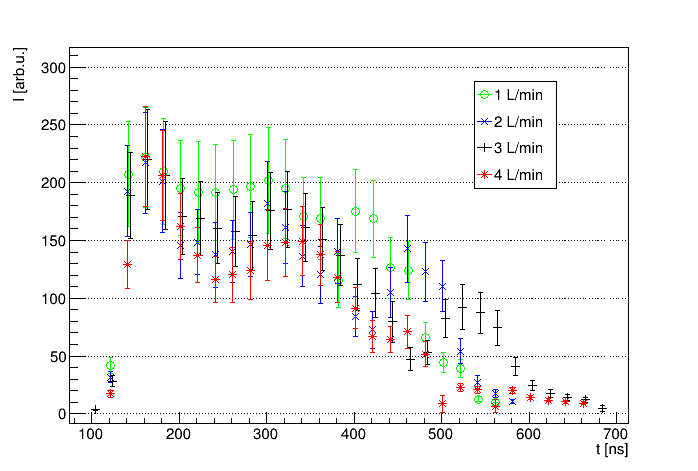
\includegraphics[width=0.48\textwidth]{Images/Shape/elio_035_Im.png}
 }
 
 \subfloat[x barycenter.]{
    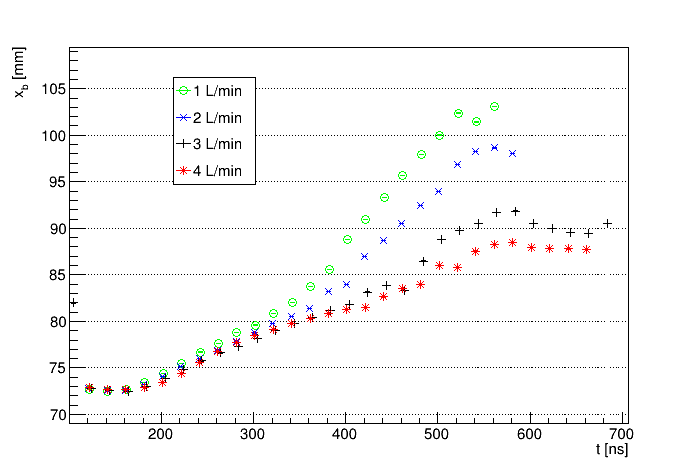
\includegraphics[width=0.48\textwidth]{Images/Shape/elio_035_xb.png}
 }
 \hfill
 \subfloat[y barycenter.]{
    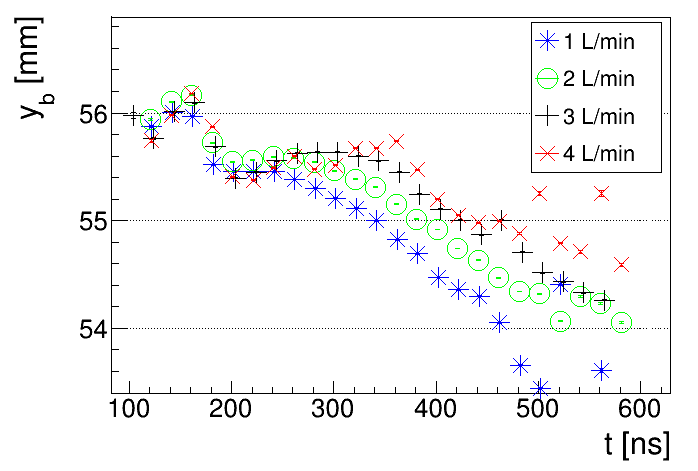
\includegraphics[width=0.48\textwidth]{Images/Shape/elio_035_yb.png}
 }
 
 \subfloat[x diameter.]{
    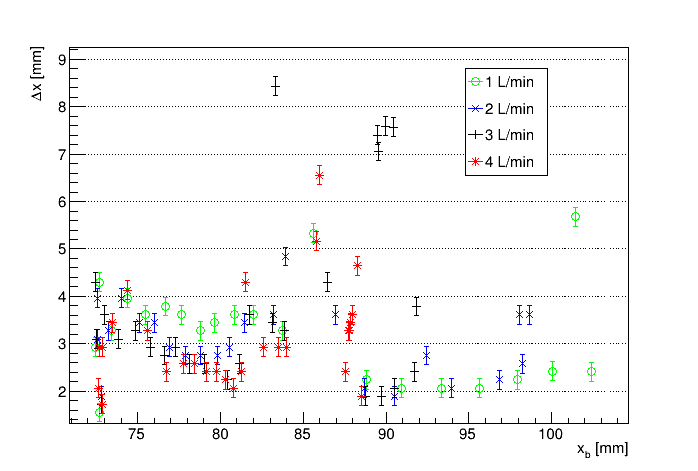
\includegraphics[width=0.48\textwidth]{Images/Shape/elio_035_dx.png}
 }
 \hfill
 \subfloat[y diameter.]{
    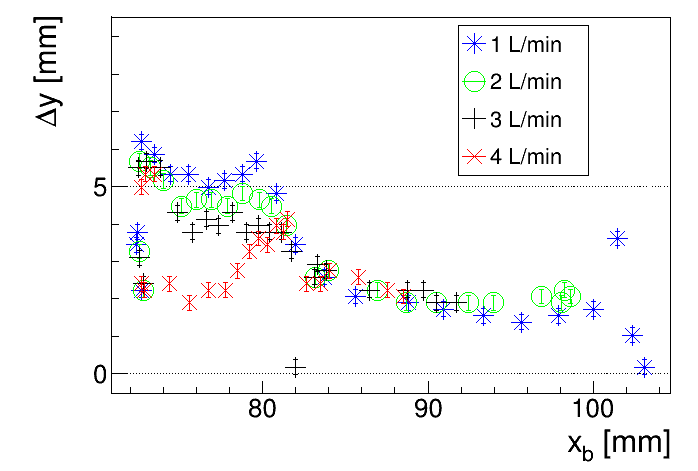
\includegraphics[width=0.48\textwidth]{Images/Shape/elio_035_dy.png}
 }
 
 \subfloat[x velocity.]{
    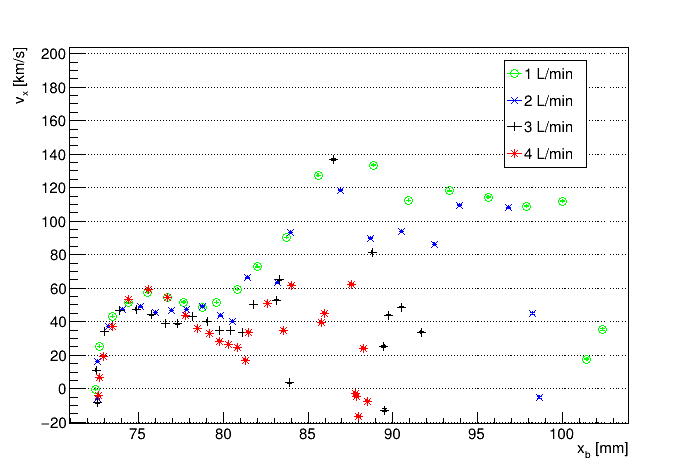
\includegraphics[width=0.48\textwidth]{Images/Shape/elio_035_vx.png}
 }
 \hfill
 \subfloat[x velocity inside the nozzle.]{
    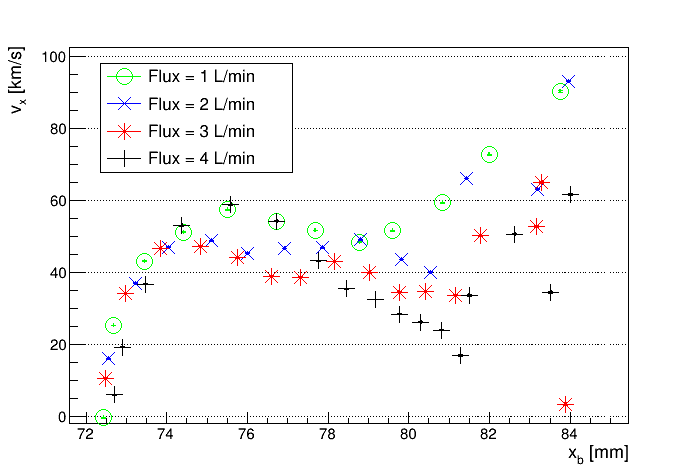
\includegraphics[width=0.48\textwidth]{Images/Shape/vnoz_flux_zoom.png}
 }
 \caption{Results of the analysis for setup A, B, C and D: different gas flow, voltage peak value of \SI{5.7}{\kilo\volt}, without target.}
 \label{fig:elio_flow}
\end{figure}

\begin{table}
 \centering
 \begin{tabular}{cccccc}
 \toprule
 Flow [L/min]    &$V_{0}$ [kV]    &$x_{\text{dist}}$ [mm]   &$y_{\text{dist}}$ [mm]   &$v_{N}$ [km/s]   &$v_{A}$ [km/s]\\
 \midrule
 \num{1}  &\num{5.87(8)}    &\num{30.65(3)} &\num{2.75(1)}  &\num{54.33(10)} &\num{113.97(9)}\\
 \num{2}  &\num{5.71(29)}    &\num{26.08(2)} &\num{1.92(4)}  &\num{46.48(2)} &\num{95.16(6)}\\
 \num{3}  &\num{5.41(27)}    &\num{19.38(1)} &\num{1.84(1)}  &\num{39.88(4)} &\num{80.96(30)}\\
 \num{4}  &\num{5.90(12)}    &\num{22.80(3)} &\num{2.30(1)}  &\num{58.89(14)} &\num{41.94(44)}\\
 \bottomrule
 \end{tabular}
 \caption{Results of the analysis for setup A, B, C and D: different gas flow, voltage peak value of \SI{5.7}{\kilo\volt}, without target. $V_{0}$ is the voltage value at plasma formation time, $x_{\text{dist}}$ and $y_{\text{dist}}$ are the highest distances reached by the bullet from electrode position, $v_{N}$ is the average velocity in x direction inside the nozzle, $v_{A}$ is the average velocity of propagation in air in x direction.}
 \label{tab:elio_d}
\end{table}


The different behavior of the bullet with different neutral gas flow could be related to the variation of the Reynold number of the fluid, that could assume critical values. Following the study in \cite{doi:10.1063/1.4819246} the Reynold number with different flow can be evaluated as in equation \ref{eq:Re}, where $v$ is the gas velocity found from the gas flow value $Q$, $\rho$ is helium density, $\mu$ is helium viscosity and $D$ is the nozzle diameter.
\begin{equation}
 \text{Rn} = \frac{v \rho D}{\mu} = \frac{Q}{\pi (D/2)^2} \frac{\rho D}{\mu}
 \label{eq:Re}
\end{equation}
Resulting values are presented in table \ref{tab:elio_Re}, always below critical Reynold number ($> \num{2000}$), there is not transition from laminar to turbolent flow for changes on neutal gas flow from \num{1} to \SI{4}{\liter/\minute}.
\begin{table}
  \centering
  \begin{tabular}{cccc}
  \toprule
  Q [L/min]   &$v_{N,\text{min}}$ [km/s]   &$x_{\text{air}}$ [\si{\milli\meter}]   &Rn\\
  \midrule
  1    &\num{48.46}    &\num{78.78}     &\num{36.88}\\
  2    &\num{40.09}    &\num{80.55}     &\num{73.77}\\
  3    &\num{33.74}    &\num{81.75}     &\num{110.65}\\
  4    &\num{17.01}    &\num{81.28}     &\num{147.54}\\
  \bottomrule
  \end{tabular}
  \caption{Bullet propagation parameters inside the nozzle for different neutral gas flow. $v_{N}$ is the lowest velocity reached inside the nozzle; $x_{\text{air}}$ is the position where the bullet increases velocity, tought to be where the bullet meets the air outside the nozzle; Rn is the Reynold number associated to the gas flow.}
  \label{tab:elio_Re}
\end{table}

While the bullet propagates inside the nozzle, at a certain time it meets the air outside, changing the elements that partecipates in ionization reactions from helium to those found in air. The bullet decelerate inside the nozzle and accelerate when it meets air (\cite{Jarrige_2010}).
The change in bullet velocity when there is an increase in neutral gas velocity could be related to the different transition time and position from helium to air. With an higher flow the bullet travels in a gas of almost only helium for longer time and its velocity decreases more, leading to a different dynamic during propagation in air.


\begin{comment}
\begin{table}
 \centering
 \begin{tabular}{ccccccc}
 \toprule
 Flow [L/min]    &$t_{0}$ [ns] &$V_{0}$ [kV]    &$x_{\text{dist}}$ [mm]   &$y_{\text{dist}}$ [mm]   &$v_{N}$ [km/s]   &$v_{A}$ [km/s]\\
 \midrule
 \num{1}  &\num{121.9}  &\num{5.87(8)}    &\num{30.65(3)} &\num{2.75(1)}  &\num{54.33(10)} &\num{113.97(9)}\\
 \num{2}  &\num{120.9}  &\num{5.71(29)}    &\num{26.08(2)} &\num{1.92(4)}  &\num{46.48(2)} &\num{95.16(6)}\\
 \num{3}  &\num{124.0}  &\num{5.41(27)}    &\num{19.38(1)} &\num{1.84(1)}  &\num{39.88(4)} &\num{40.96(10)}\\
 \num{4}  &\num{121.3}  &\num{5.90(12)}    &\num{22.80(3)} &\num{2.30(1)}  &\num{58.89(14)} &\num{61.94(44)}\\
 \bottomrule
 \end{tabular}
 \caption{Result of the analysis with different gas flows. $t_{0}$ is the bullet formation time, $V_{0}$ the bullet formation tension, $x_{\text{dist}}$ and $y_{\text{dist}}$ are the highest distances reached by the bullet from electrode position, $v_{N}$ is the velocity in x direction reached inside the nozzle, $v_{A}$ is the velocity of propagation in air in x direction.}
 \label{tab:elio_d}
\end{table} 
\end{comment}


\subsection{Insulating target}
The electric field created by the electrode is not expected to change if there is an insulating target in front of the nozzle. An intersting effect is seen after the bullet impacts on the target, as shown in figure \ref{fig:elio_ins}: plasma forms a round shaped figure on the insulator that enlarges on the target until the luminosity decreases.
\begin{comment}
\begin{figure}
 \centering
 \subfloat[Bullet propagation \SI{437.6}{\nano\second}.]{
    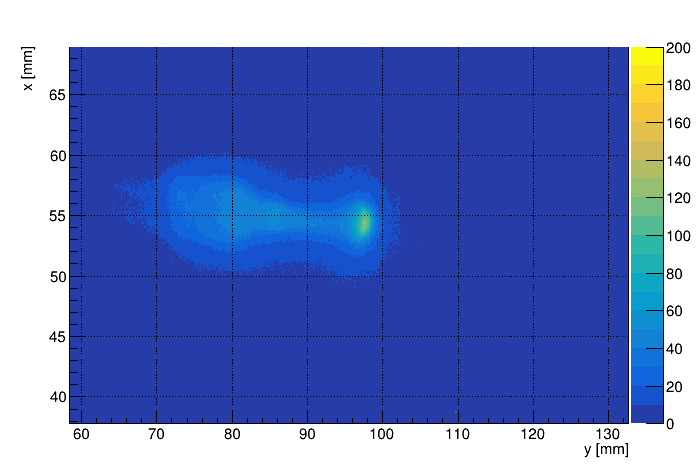
\includegraphics[width=0.42\textwidth]{Images/Shape/elio_ins1.png}
 }
 \hfill
 \subfloat[Bullet impact \SI{457.6}{\nano\second}.]{
    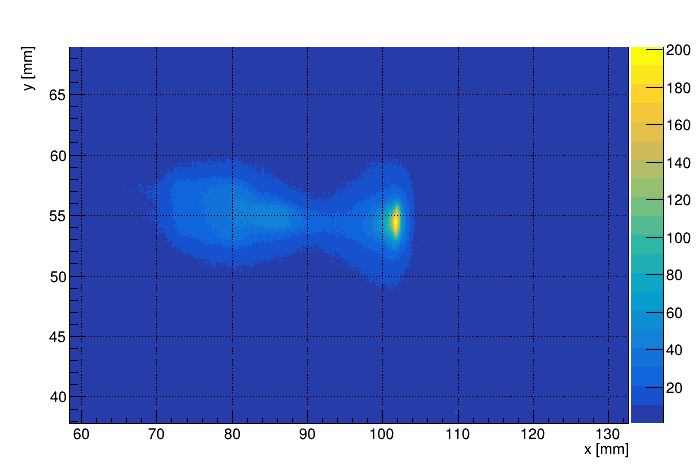
\includegraphics[width=0.42\textwidth]{Images/Shape/elio_ins2.png}
 }
 \hfill
 \subfloat[Charge deposition \SI{577.6}{\nano\second}.]{
    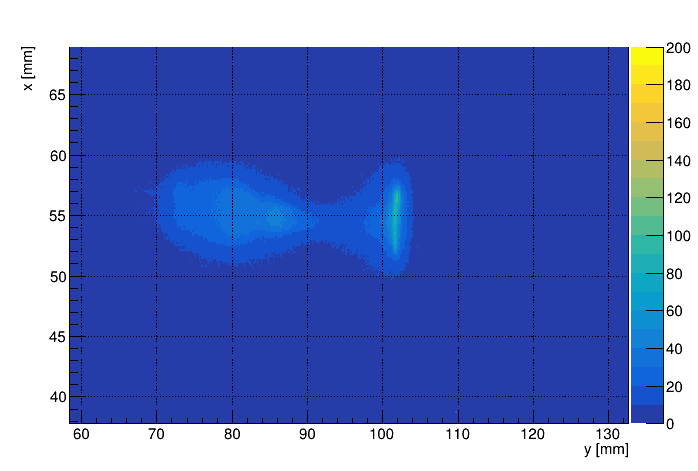
\includegraphics[width=0.42\textwidth]{Images/Shape/elio_ins3.png}
 }
 \caption{Impact and charge deposition on an insulator target, measurements setup E.}
 \label{fig:elio_ins}
\end{figure}
\end{comment}
\begin{figure}
 \centering
 \subfloat[Picture of the setup.]{
    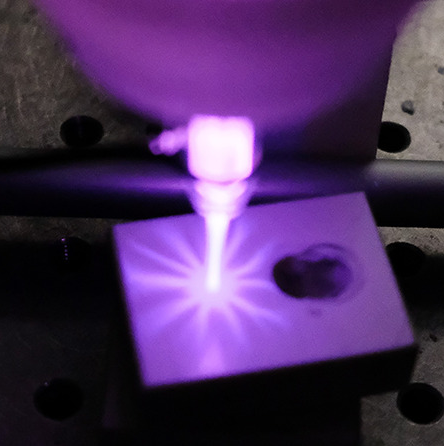
\includegraphics[width=0.48\textwidth]{Images/Shape/elioisol.png}
 }
 \hfill
 \subfloat[Frame showing bullet on target impact.]{
    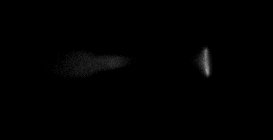
\includegraphics[width=0.48\textwidth]{Images/Shape/elioisol_frame2.png}
 }
 \caption{Impact of plasma on an insulating target. In (a) picture of the plume, in (b) frame acquisited for setup E, voltage peak \SI{7.2}{\kilo\volt}.}
 \label{fig:elio_ins}
\end{figure}


Barycenter x coordinate of the bullet and its diameter are presented in figure \ref{fig:elio_c_xb}. While for the lowest tension value the bullet stops before it reaches the target, for the other two sets it clearly stops at the target position. Distance values are comparable with those without target (figure \ref{fig:elio_d}), higher for medium voltage value.
Bullet width is exactly the same with or without target, it shows differences only when it impacts on the target and shrinks rapidly.
Displacement velocities inside the nozzle and propagation velocities in air are of the same order of values without target, shown figure \ref{fig:elio_c_vx}. There is higher $v_{A}$ only for medium tension value, where it reaches \SI{118.98(7)}{\kilo\meter/\second}, due to the rapid collision with the target instead of slowing down and stopping.
\begin{figure}
 \centering
 \subfloat[Barycenter position.]{
    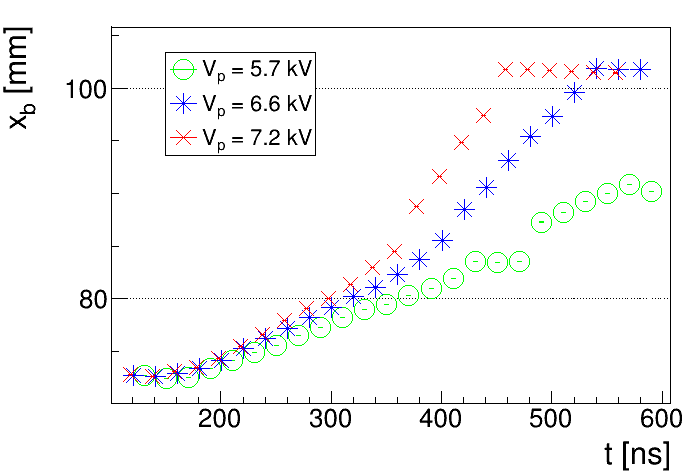
\includegraphics[width=0.48\textwidth]{Images/Shape/elio_c_xb.png}
 }
 \hfill
 \subfloat[Bullet diameter.]{
    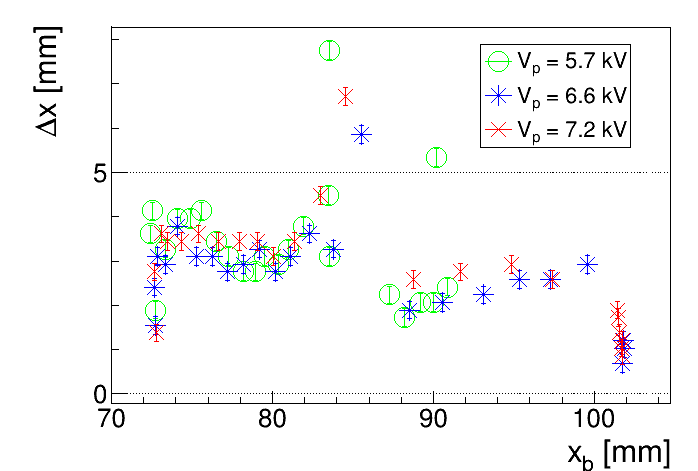
\includegraphics[width=0.48\textwidth]{Images/Shape/elio_c_dx.png}
 }
 \caption{Barycenter motion and diameter in x direction for measurements setup E (presence of insulating target) for different voltage peak values.}
 \label{fig:elio_c_xb}
\end{figure}

\paragraph{Charge deposition}
Once the bullet reaches the target it is possible to see how the glowing region enlarges on its surface and the bullet diameter increases, as shown in figure \ref{fig:elio_c_ylim}. Is possible to evaluate the expansion diameter and velocity observing bullet contour in the y direction once the bullet reaches the target. In figure \ref{fig:elio_c_ylim} can be seen that the diameter and the expansion velocity are higher for higher voltage value: for a voltage peak of \SI{6.6}{\kilo\volt} the shape on the insulator has a maximum diameter of \SI{6.54(4)}{\milli\meter} and an expansion velocity of \SI{31.36(25)}{\kilo\meter/\second}; for \SI{7.2}{\kilo\volt} the values are \SI{7.40(2)}{\milli\meter} and \SI{64.04(39)}{\kilo\meter/\second}. %The bullet has higher velocity along x so it is possible that it has also higher expansion velocity on the target, reaching further distances.
\begin{figure}
 \centering
 \subfloat[Bullet diameter.]{
    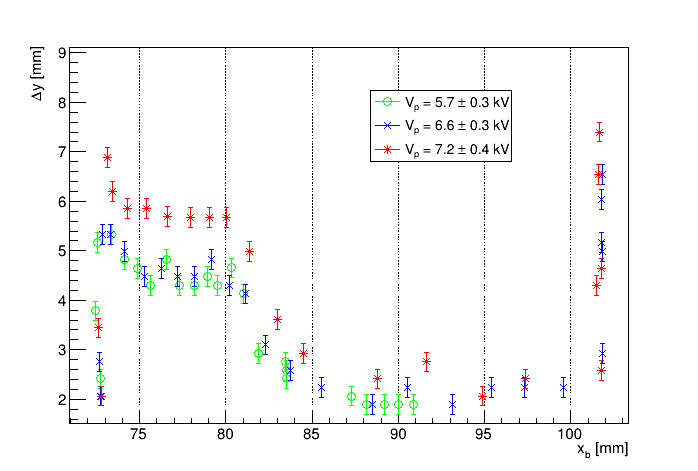
\includegraphics[width=0.48\textwidth]{Images/Shape/elio_c_dy.png}
 }
 \hfill
 \subfloat[Bullet expansion in time.]{
    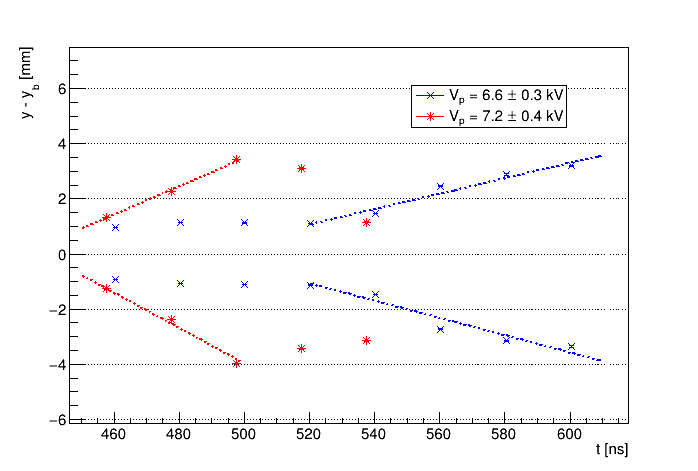
\includegraphics[width=0.48\textwidth]{Images/Shape/elio_c_ylim.png}
 }
 \caption{Charge deposition in y direction on an insulating target, for measurements setup E. In (a) there is the absolute value for the diameter for all barycenter positions; in (b) the expansion of y contour after it reaches the target for medium and high voltage peak value. Contour values are calculated as difference with the barycenter y coordinate, linear fits show how much the diameter enlarges in time.}
 \label{fig:elio_c_ylim}
\end{figure}


\subsection{Conductive target}
A grounded conductive target could influence bullet propagation because it fixs the value of the electric field on that point in space and it presents free charges on its surface.
In measurements setup F and G a conductive target is positioned in two different positions.

For measurement setup F a conductive target is positioned at \SI{24}{\milli\meter} from the bench, correponding to \SI{30}{\milli\meter} from the electrode. 

%This target allows to measure current intensity flowing in it and is possible to compare the bullet impact time with the starting time of the peak current.  the relation between bullet and current flowing in the target. 
When the bullet impacts on the conductive target can be observed a rapid increase in luminosity on the target and in the space between nozzle and target as shown in figure \ref{fig:elio_met}. In this work it will be referred as ``backstream'' (because it seems to have motion inverse to that of the bullet). Analysis of bullet propagation, impact and evolution on target is treated separately from analysis of backstream, to allow comparision with other measurements setup.
\begin{figure}
 \centering
 \subfloat[Bullet propagation \SI{371.2}{\nano\second}.]{
    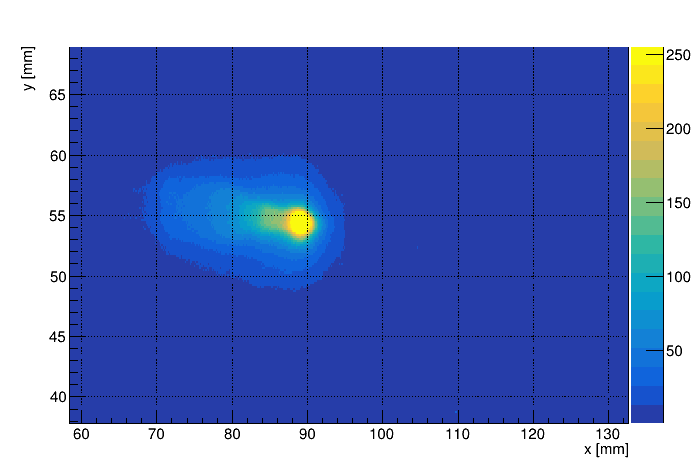
\includegraphics[width=0.42\textwidth]{Images/Shape/elio_met1.png}
 }
 \hfill
 \subfloat[Bullet impact \SI{391.2}{\nano\second}.]{
    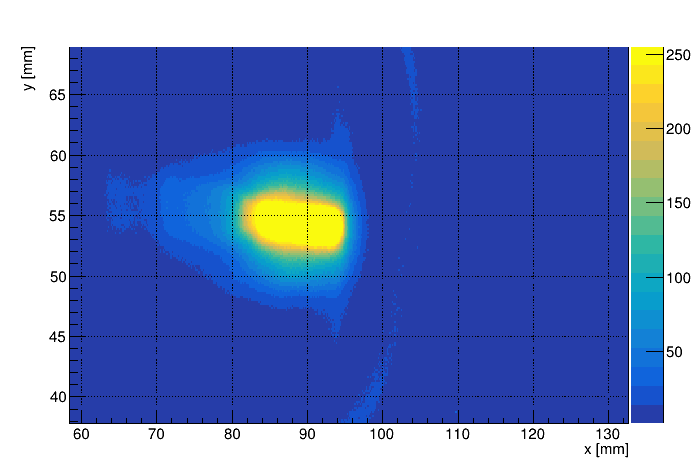
\includegraphics[width=0.42\textwidth]{Images/Shape/elio_met2.png}
 }
 \hfill
 \subfloat[Backstream \SI{411.2}{\nano\second}.]{
    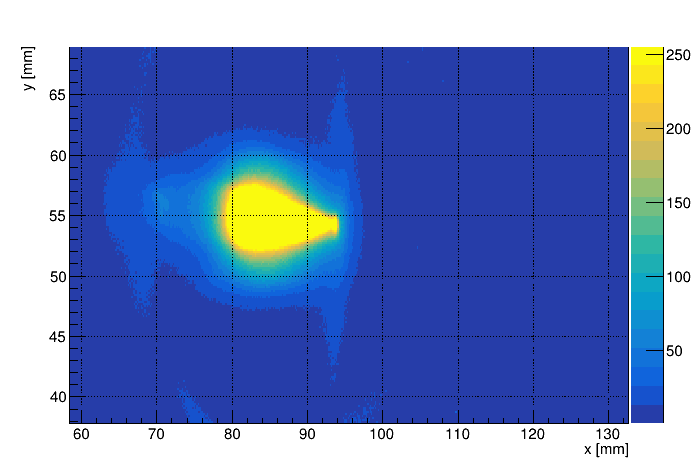
\includegraphics[width=0.42\textwidth]{Images/Shape/elio_met3.png}
 }
 \caption{Example of frames showing impact on a conductive target and consequent backstream, measurements setup F with voltage peak value \SI{7.2}{\kilo\volt}.}
 \label{fig:elio_met}
\end{figure}


\paragraph{Bullet dynamics}
Bullet propagation is different if compared to measurements without conductive target. From figure \ref{fig:elio_a_Im} is possible to see that bullet luminosity presents an increase in correspondence of the second voltage peak (negative). This results in an increase of bullet lifetime up to \SI{900}{\nano\second} from the first voltage peak.
\begin{figure}
 \centering
 \subfloat[Voltage waveforms.]{
    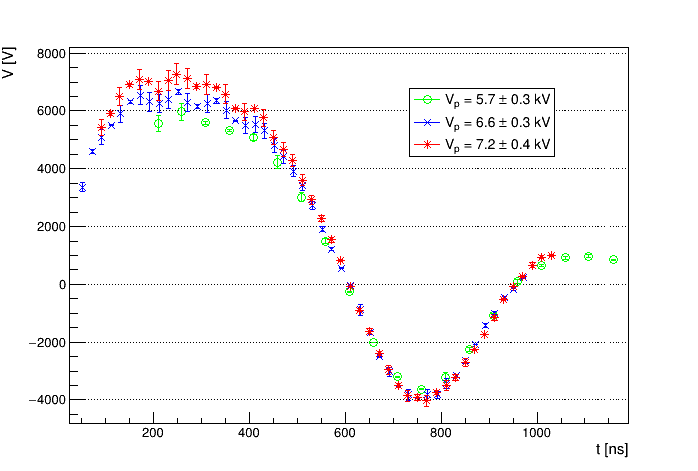
\includegraphics[width=0.43\textwidth]{Images/Shape/elio_a_V.png}
 }
 \hfill
 \subfloat[Bullet luminosity.]{
    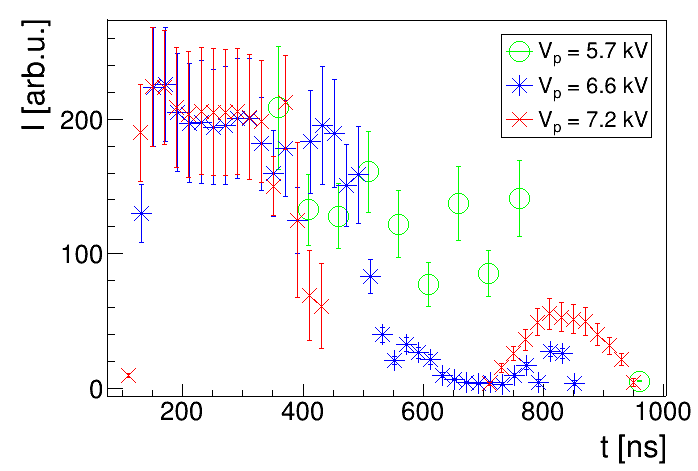
\includegraphics[width=0.43\textwidth]{Images/Shape/elio_a_Im.png}
 }
 \caption{Voltage on the elctrode and bullet luminosity for measurements setup F, different peak voltage values. Note the second luminosity peak in correspondence of the negative voltage peak.}
 \label{fig:elio_a_Im}
\end{figure}

Barycenter motions shows that even with low voltage the bullet reaches the target, different from the behavior with the insulating target. Propagation velocity is higher then values found in other configurations.
Bullet diameter doesn't shows different behaviour, it stays constant until nozzle exit and remains constant until it reaches the target and shrinks to a point. As said before, velocities of propagation in air are generally larger then whitout target, they arrives from \SI{112.04(5)}{\kilo\meter/\second} for low voltage peak to \SI{160.55(9)}{\kilo\meter/\second} for high voltage peak.
\begin{figure}
 \centering
 \subfloat[Barycenter.]{
    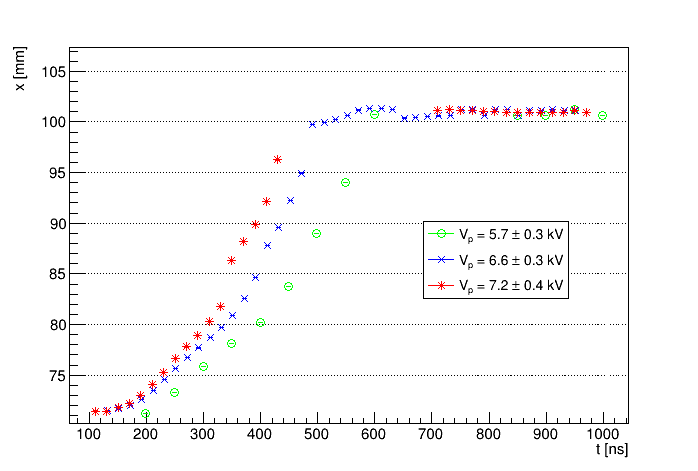
\includegraphics[width=0.43\textwidth]{Images/Shape/elio_a_xb.png}
 }
 \hfill
 \subfloat[Diameter.]{
    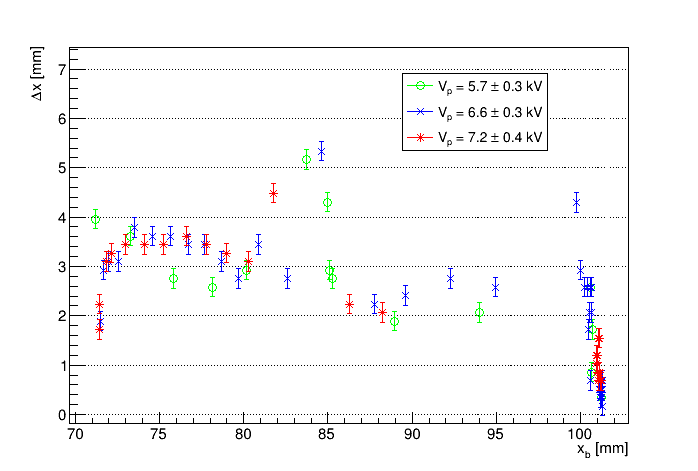
\includegraphics[width=0.43\textwidth]{Images/Shape/elio_a_dx.png}
 }
 \subfloat[Velocity.]{
    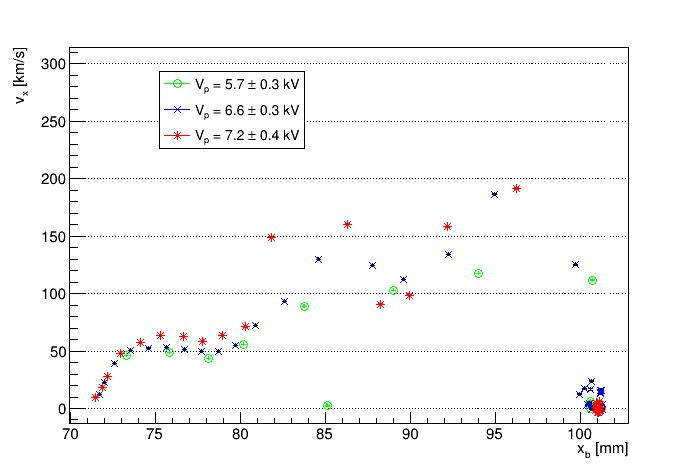
\includegraphics[width=0.43\textwidth]{Images/Shape/elio_a_vx.png}
 }
 \caption{Bullet barycenter coordinate, diameter and velocity along x direction, for measurement setup F and for different peak voltage values. Can be seen as the bullet reaches the target, it shrinks and stops.}
 \label{fig:elio_a_xb}
\end{figure}

\paragraph{Current measurements}
Current intensity flowing in the conductive target due to charge transported by plasma can be measured. The correlation between bullet and charge deposition can be verified observing the relation between impact time and peak current starting time.

Current intensity it's shown in figure \ref{fig:elio_a_icurr}, it presents two peaks, a positive one and a negative one. For the lowest voltage value current peaks are not high enough to analyze them, this set is excluded from the following analysis.
The positive peak value starts at time $t_{0,i}$ and reaches the maximum at time $t_{0,i}$. Both values are inversely proportional to voltage peak value, we have lower and slower current intensity when the voltage is lower. Those times can be compared with the impact time of the bullet on the target, $t_{\text{imp}}$, in table \ref{tab:elio_a_times} are presented the values. 
It is possible to see that current starts flowing into the target before the bullet reaches the target, and even maximum current is measured before the impact time of the bullet.
It's also intersting to evaluate the distance of bullet from target when we measure current, in table \ref{tab:elio_a_times} there is the difference between bullet barycenter position and target position $x_{\text{target}} - x(t_{0,i})$.


%The first positive peak is not  can see a positive peak, more influenced by tension peak value, and a negative peak in correspondence of the negative tension peak and of the second luminosity peak for the bullet. It's important to note that the time interval where we have high luminosity for the bullet and its position is around the target position, is the same time interval where we measure current.
\begin{figure}
 \centering
 \includegraphics[width=0.6\textwidth]{Images/Shape/elio_a_icurr.png}
 \caption{Current intensity for measurements setup F, for different voltage peak values.}
 \label{fig:elio_a_icurr}
\end{figure}
\begin{table}
 \centering
 \begin{tabular}{cccccc}
  \toprule
  $V_{p}$ [kV]  &$i_{p}$ [mA]   &$t_{0,i}$ [ns] &$t_{p,i}$ [ns] &$t_{\text{imp}}$ [ns]  &$x_{\text{target}} - x(t_{0,i})$ [mm]\\
  \midrule
  %\num{5.7(3)}  &\num{17.56(88)}    &\num{459.1(150)}   &\num{509.2(150)}   &\num{499.1(150)}   &\num{7.20(1)}\\
  \num{6.6(3)}  &\num{32.63(163)}    &\num{391.6(150)}   &\num{451.6(150)}   &\num{511.6(150)}   &\num{9.22(1)}\\
  \num{7.2(4)}  &\num{41.50(62)}    &\num{350.3(150)}   &\num{410.3(150)}   &\num{450.3(150)}   &\num{15.18(2)}\\
  \bottomrule
 \end{tabular}
 \caption{Results of the analysis of current measurements for setup F. $V_{p}$ is the voltage peak for the pulse, $i_{p}$ is the current peak value, $t_{0,i}$ is the starting time for the current pulse, $t_{p,i}$ is the maximum current time, $t_{\text{imp}}$ is the time impact of bullet on target, $x_{\text{target}} - x(t_{0,i})$ is the distance between bullet position when we start to measure current and target position.}
 \label{fig:elio_a_times}
\end{table}

Those results could be explained by the presence of ionized particles that does not produce reactions with emission at visible wavelengths. Current would be measured even without seeing the impact of plasma on the target if the bullet has a diameter higher then the one measurable with the camera. This invisible portion of the bullet would have the same behavior of the bullet for different voltage values, i.e. it would increase its velocity with higher voltage. As can be seen from table \ref{tab:elio_a_times} the current peak starts indeed before with higher voltage.

%The ratio between nozzle velocities with different voltage values gives an estimation on how velocity changes increasing voltage, from table \ref{tab:elio_d} it is \num{0.78(1)}. If the starting time of the peak current is related to bullet motion the ratio between those times would be a comparable value with the ratio of velocities. From table \ref{tab:elio_a_times} we find  

\paragraph{Backstream}
Dynamics of the backstream is difficult to analyze as it's a rapid phenomenon with too high luminosity. Frames right after the impact of the bullet on target present another zone with high luminosity right after nozzle exit. This other glow has stable position and diameter, as can be seen in figure \ref{fig:elio_a_back}, with a slow tendency to shift towards the target when voltage is positive and towards the electrode when it's negative.
The phenomenon can be explained as a very rapid charge stream from the target to the electrode, that stops when meets the nozzle, but to study it are necessary other specific measures with more time resolution.
\begin{figure}
 \centering
 \subfloat[Mean luminosity.]{
    \includegraphics[width=0.43\textwidth]{Images/Shape/elio_a_Im_back.png}
 }
 \hfill
 \subfloat[Barycenter along x.]{
    \includegraphics[width=0.43\textwidth]{Images/Shape/elio_a_xb_back.png}
 }
 
 \subfloat[Diameter along x.]{
    \includegraphics[width=0.43\textwidth]{Images/Shape/elio_a_dx_back.png}
 }
 \hfill
 \subfloat[Diameter along y.]{
    \includegraphics[width=0.43\textwidth]{Images/Shape/elio_a_dy_back.png}
 }
 \caption{Backstream analysis for measurements setup F. It's possible to see the decreasing luminosity while the barycenter stays around the nozzle exit and diameter stays constant.}
 \label{fig:elio_a_back}
\end{figure}


\subsubsection{Position of the target}
The position of the target could influence bullet propagation. In measurement setup G the conductive target is positioned at \SI{32}{\milli\meter} from the bench, correponding to \SI{22}{\milli\meter} from the electrode, closer to the nozzle respect setup F.

With a conductive target this close it's more difficult to see the bullet evolution, as it is more rapid and the backstream has even higher relevance.

In figure \ref{fig:elio_b_dyn} are presented the results of the analysis. For all the sets there is high luminosity, even after a time interval corresponding to the end of the voltage peak.
For higher voltage peak values, it is not possible to see the bullet, as it reaches the target in a sort of large plume right after nozzle exit. The other two sets shows the same behaviour described before, with even higher velocities: for medium voltage velocity inside the nozzle velocity is \SI{59.30(5)}{\kilo\meter/\second}, while maximum velocity in air is \SI{174.44(8)}{\kilo\meter/\second}.
\begin{figure}
 \centering
 \subfloat[Mean luminosity.]{
    \includegraphics[width=0.43\textwidth]{Images/Shape/elio_b_Im.png}
 }
 \hfill
 \subfloat[Barycenter along x.]{
    \includegraphics[width=0.43\textwidth]{Images/Shape/elio_b_xb.png}
 }
 
 \subfloat[Diameter along x.]{
    \includegraphics[width=0.43\textwidth]{Images/Shape/elio_b_dx.png}
 }
 \hfill
 \subfloat[Diameter along y.]{
    \includegraphics[width=0.43\textwidth]{Images/Shape/elio_b_vx.png}
 }
 \caption{Analysis of measurement setup G: conductive target positioned close to the nozzle.}
 \label{fig:elio_b_dyn}
\end{figure}

\paragraph{Current measurements}
As done with previous setup, for low and medium voltage it's possible to analyze time and space intervals between bullet barycenter motion and current measurements. Obtained values are shown in table \ref{tab:elio_b_times}.
\begin{table}
 \centering
 \begin{tabular}{cccccc}
  \toprule
  $V_{p}$ [kV]  &$i_{p}$ [mA]   &$t_{0,i}$ [ns] &$t_{p,i}$ [ns] &$t_{\text{imp}}$ [ns]  &$x_{\text{target}} - x(t_{0,i})$ [mm]\\
  \midrule
  \num{5.7(3)}  &\num{47.41(237)}    &\num{370.6(150)}   &\num{450.6(150)}   &\num{450.6(150)}   &\num{11.34(2)}\\
  \num{6.6(4)}  &\num{77.41(387)}    &\num{311.2(150)}   &\num{411.2(150)}   &\num{391.2(150)}   &\num{13.61(4)}\\
  \bottomrule
 \end{tabular}
 \caption{Values extrapolated from current measurements and bullet barycenter motion for setup G. $V_{p}$ is the voltage peak for the pulse, $i_{p}$ is the current peak value, $t_{0,i}$ is the starting time for the current value, $t_{p,i}$ is the time of current peak value, $t_{\text{imp}}$ is the time of the impact of bullet on target, $x_{\text{target}} - x(t_{0,i})$ is the distance between bullet position when current peak starts and target position.}
 \label{fig:elio_a_times}
\end{table}

Again current flows in target before the impact of the bullet, when it is distant from the target (parameter $x_{\text{target}} - x(t_{0,i})$ in table). Comparing these values with results for setup F, is possible to see that for the same voltage peak value, the current peak starts faster and reaches an higher peak value. Hypotizing that charge motion is correlated to bullet motion an earlier impact point means that the bullet will lose less charge during the propagation in air and that there will be higher current intensity flowing on target.


\section{Neon flow}
The second noble gas used to produce cold plasma is neon, the one with more emission intensity at visible wavelength.
Neon it's an element with standard atomic weight of $\num{20.180}$, 1st ionization energy of \SI{21.565}{\electronvolt} and 2nd ionization energy of \SI{40.963}{\electronvolt} and several lines with wavelength in visible spectrum. It's easy to produce neon plasma, when the voltage pulse is applied, even with low repetition rates, the gas presents high luminosity in a wide space. This emissivity it's the reason why neon is commonly used to build neon lamps.

The working pulse repetition rate is set to $f = \SI{1}{\kilo\hertz}$ and three opening times equivalent to low, medium and high voltage in helium. Different measurement setup are presented in table \ref{tab:setups}.

\subsection{Free bullet}
First measurements are done to see plasma dynamics whitout a target, changing between low, medium and high tension peak value. Results are shown in figure \ref{fig:neon_d} and table \ref{tab:neon_d}.
First thing to notice is that plasma is produced not specifically at electrode's end where the electric field should be higher, as in helium, but a little before, with lower luminosity. Luminosity evolution from there is similar to that of helium bullet, but there is a residual luminosity tail that lasts longer.
Barycenter motion and diameter evolution present the same evolution of helium bullets inside the nozzle. Outside the nozzle there are two main differences:
\begin{itemize}
 \item neon bullets come out of the nozzle more difficultly and lose velocity more rapidly, covering shortest distances. Propagation velocity in air rises exiting the nozzle (until \SI{160.32(7)}{\kilo\meter/\second} with high voltage), but goes down abruptily and the bullet slows down rapidly.
 \item neon bullet's x diameter rises increasing voltage. As can be seen from figure \ref{fig:neon_s}, diameter evolution is the same as in helium bullet, but there are higher diameter values with higher voltage.
\end{itemize}

Those differences can be explained by the different reactions that have place in neon plasma. If those reactions need less energetic electrons, we would have more of them that partecipates, increasing the diameter of the bullet.
\begin{figure}
 \centering
 \subfloat[Voltage waveform.]{
    \includegraphics[width=0.46\textwidth]{Images/Shape/neon_a_V.png}
 }
 \hfill
 \subfloat[Mean luminosity.]{
    \includegraphics[width=0.46\textwidth]{Images/Shape/neon_d_Im.png}
 }
 
 \subfloat[x barycenter.]{
    \includegraphics[width=0.46\textwidth]{Images/Shape/neon_d_xb.png}
 }
 \hfill
 \subfloat[x velocity.]{
    \includegraphics[width=0.46\textwidth]{Images/Shape/neon_d_vx.png}
 }
 
 \subfloat[x diameter.]{
    \includegraphics[width=0.46\textwidth]{Images/Shape/neon_d_dx.png}
 }
 \hfill
 \subfloat[y diameter.]{
    \includegraphics[width=0.46\textwidth]{Images/Shape/neon_d_dy.png}
 }
 \caption{Results of the analysis for measurement setup A with neon gas, for different peak voltage values.}
 \label{fig:neon_d}
\end{figure}


\begin{table}
 \centering
 \begin{tabular}{ccccc}
 \toprule
 $V_{p}$ [kV]    &$V_{0}$ [kV]    &$x_{\text{dist}}$ [mm]   &$v_{N}$ [km/s]   &$v_{A}$ [km/s]\\
 \midrule
 \num{4.81(24)}  &\num{4.81(24)}    &\num{18.13(5)} &\num{34.59(3)} &\num{43.19(7)}\\
 \num{5.33(27)}  &\num{5.20(26)}    &\num{22.42(6)} &\num{42.82(4)} &\num{61.17(5)}\\
 \num{6.05(30)}  &\num{5.16(26)}    &\num{26.60(9)} &\num{62.92(5)} &\num{160.32(7)}\\
 \bottomrule
 \end{tabular}
 \caption{Results of the analysis for measurements setup A with neon, for different voltage peak values. $V_{p}$ is the peak value for the pulse, $V_{0}$ bullet formation tension, $x_{\text{dist}}$ is the highest distances reached by the bullet from electrode position, $v_{N}$ is the velocity in x direction reached inside the nozzle, $v_{A}$ is the velocity of propagation in air.}
 \label{tab:neon_d}
\end{table}


For both helium and neon inside the nozzle there is bullet propagation, it is possible to compare how the velocity $v_{N}$ changes varying voltage peak value for the gasses. In figure \ref{fig:hene_d_vn} there is the plot for the two gasses. With few points it's not possible to extrapolate accurately the behavior, but a linear plot shows that helium bullet's velocity grows with a slope of \SI{14.55(240)}{\kilo\meter/\second \kilo\volt}, while neon bullet's velocity has a slope of \SI{23.23(366)}{\kilo\meter/\second \kilo\volt}. Those values are of the same magnitude, but not compatible, suggesting that bullet's velocity may depend from gas composition.
\begin{figure}
 \centering
 \includegraphics[width=0.52\textwidth]{Images/Shape/hene_vN.png}
 \caption{Bullet velocity inside the nozzle as a function of voltage peak value, for helium and neon.}
 \label{fig:hene_d_vn}
\end{figure}


\subsection{Insulating target}
Also for neon is studied the dynamic with an insulating target positioned at \SI{30}{\milli\meter} from the electrode, in measurement setup B.
Results are similar with helium or neon bullets: palsma forms near the electrode, exits from the nozzle and the impact on the target produce a round shaped figure on it, as in figure \ref{fig:elio_ins}. Also in neon for low voltage peak value the bullet doesn't reaches the target, as the maximum distance travelled is lower then target distance. This suggests that the target does not influences the bullet when it is not in its proximity.
A peculiarity with neon is that there is a second, very low, peak in luminosity corresponding to the second voltage peak of the pulse.
\begin{figure}
 \centering
 \subfloat[Mean luminosity.]{
    \includegraphics[width=0.46\textwidth]{Images/Shape/neon_c_dx.png}
 }
 \hfill
 \subfloat[Barycenter position.]{
    \includegraphics[width=0.46\textwidth]{Images/Shape/neon_c_xb.png}
 }
 \caption{Mean luminosity and barycenter motion for neon gas in setup measuerement D.}
 \label{fig:neon_c_xb}
\end{figure}


The figure that bullet impact produces on target can be analyzed as with helium. In figure \ref{fig:neon_c_ylim} there is the y contour in function of time and is possible to extrapolate an expansion velocity of \SI{5.01(29)}{\kilo\meter/\second} for medium voltage and \SI{30.76(25)}{\kilo\meter/\second} for high voltage. They are both lower compared to helium, probably because the bullet in neon slows down more rapidly once it's outside the nozzle.
\begin{figure}
 \centering
 \includegraphics[width=0.46\textwidth]{Images/Shape/neon_c_ylim.png}
 \caption{Neon plasma expansion on insulator target, measurements setup B for different voltage peak values.}
 \label{fig:neon_c_ylim}
\end{figure}


\subsection{Conductive target}
As with helium, a conductive target has an influence in all neon bullet's dynamics. If compared to helium the bullet goes more rapidly from a round shape to the elongated one that gives rise to the backstream described in figure \ref{fig:elio_met}.

In figure \ref{fig:neon_ab_xb} is possible to see that the distant target (setup C) is reached by the bullet with medium and high voltage, but there isn't a change in luminosity. Near nozzle exit the bullet speeds up, reaches rapidly the target, stretches and then reduces its diameter to the impact point.
For a close target there is a change in luminosity in correspondence of the negative voltage peak and of the second voltage positive peak. With high voltage the bullet shape is losed completely once plasma exits the nozzle, all the space between nozzle exit and target is completely filled by glowing gas.
\begin{figure}
 \centering
 \subfloat[Mean luminosity, $\Delta x_{\text{targ}} = \SI{30}{\milli\meter}$.]{
    \includegraphics[width=0.46\textwidth]{Images/Shape/neon_a_Im.png}
 }
 \hfill
 \subfloat[Mean luminosity, $\Delta x_{\text{targ}} = \SI{22}{\milli\meter}$.]{
    \includegraphics[width=0.46\textwidth]{Images/Shape/neon_b_Im.png}
 }
 
 \subfloat[x barycenter, $\Delta x_{\text{targ}} = \SI{30}{\milli\meter}$]{
    \includegraphics[width=0.46\textwidth]{Images/Shape/neon_a_xb.png}
 }
 \hfill
 \subfloat[x barycenter, $\Delta x_{\text{targ}} = \SI{22}{\milli\meter}$]{
    \includegraphics[width=0.46\textwidth]{Images/Shape/neon_b_xb.png}
 }
 
 \subfloat[x diameter, $\Delta x_{\text{targ}} = \SI{30}{\milli\meter}$]{
    \includegraphics[width=0.46\textwidth]{Images/Shape/neon_a_dx.png}
 }
 \hfill
 \subfloat[x diameter, $\Delta x_{\text{targ}} = \SI{22}{\milli\meter}$]{
    \includegraphics[width=0.46\textwidth]{Images/Shape/neon_b_dx.png}
 }
 \caption{Results of the analysis for measurement setup C and D with neon gas, for different peak voltage values.}
 \label{fig:neon_ab_xb}
\end{figure}


\paragraph{Current measurements}
%Neon current measures are done in the same way of different from helium measurements.
In figure \ref{fig:neon_ab_icurr} ad in table \ref{tab:neon_ab_ival} there are results for the analysis of current measurements, similar to those done with helium. A current peak is measured only for high voltage with distant target and for medium and high voltage with close target. Starting time of current peak is again precedent to the impact time of the bullet with the target. Interaction distances presented in table are similar to the ones found for helium.
The absence of the current peak for medium voltage with distant target could mean that the target is not reached by the charge carrier, even if we see luminosity on the target. With higher voltage the bullet and the charge carrier are more rapid, reach the target and we measure current.
\begin{figure}
 \centering
 \subfloat[$\Delta x_{\text{targ}} = \SI{30}{\milli\meter}$.]{
    \includegraphics[width=0.46\textwidth]{Images/Shape/neon_a_i.png}
 }
 \hfill
 \subfloat[$\Delta x_{\text{targ}} = \SI{22}{\milli\meter}$.]{
    \includegraphics[width=0.46\textwidth]{Images/Shape/neon_b_i.png}
 }
 \caption{Current intensity measured for neon in setups C and D, with different voltage peak values.}
 \label{fig:neon_ab_icurr}
\end{figure}

\begin{table}
 \centering
 \begin{tabular}{ccccccc}
  \toprule
  $\Delta x_{\text{targ}}$ [mm] &$V_{p}$ [kV]  &$i_{p}$ [mA]   &$t_{0,i}$ [ns] &$t_{p,i}$ [ns] &$t_{\text{imp}}$ [ns]  &$x_{\text{target}} - x(t_{0,i})$ [mm]\\
  \midrule
  \num{30}  &\num{6.05(30)}  &\num{6.87(34)}    &\num{329(15)}   &\num{477(15)}   &\num{453(21)}   &\num{19.96(3)}\\
  \midrule
  \multirow{2}*{\num{22}}   &\num{5.33(27)}  &\num{7.72(39)}    &\num{347(15)}   &\num{447(15)}   &\num{447(15)}   &\num{13.06(3)}\\
                            &\num{6.05(30)}  &\num{14.56(73)}    &\num{300(15)}   &\num{398(15)}   &\num{380(21)}   &\num{13.66(4)}\\
  \bottomrule
 \end{tabular}
 \caption{Values extrapolated from current measure and bullet barycenter motion for neon in setups C and D. $\Delta x_{\text{targ}}$ is the distance between electrode and target, $V_{p}$ is the voltage peak for the pulse, $i_{p}$ is the current peak value, $t_{0,i}$ is the starting time for the current value, $t_{p,i}$ is the time of the peak value, $t_{\text{imp}}$ is the time of the impact of bullet on target, $x_{\text{target}} - x(t_{0,i})$ is the distance between bullet position when current peak starts and target position.}
 \label{fig:neon_ab_ival}
\end{table}


\paragraph{Backstream}
Backstream phenomenon in neon is easily observable, where the bullet reaches the target there is high luminosity around nozzle exit. It presents itself as zone of glowing gas with large width and near constant height, with a barycenter motion that shift direction towards the electrode or towards the target. The changes of barycenter coordinates in time is so low that is not possible to infer it's dynamics. Once the pulse voltage lowers, also the backstream fade away.
\begin{figure}
 \centering
 \subfloat[Mean luminosity, $\Delta x_{\text{targ}} = \SI{30}{\milli\meter}$.]{
    \includegraphics[width=0.43\textwidth]{Images/Shape/neon_a_back_Im.png}
 }
 \hfill
 \subfloat[Mean luminosity,  $\Delta x_{\text{targ}} = \SI{22}{\milli\meter}$.]{
    \includegraphics[width=0.43\textwidth]{Images/Shape/neon_b_back_Im.png}
 }
 
 \subfloat[Barycenter along x, $\Delta x_{\text{targ}} = \SI{30}{\milli\meter}$.]{
    \includegraphics[width=0.43\textwidth]{Images/Shape/neon_a_back_xb.png}
 }
 \hfill
 \subfloat[Barycenter along x,  $\Delta x_{\text{targ}} = \SI{22}{\milli\meter}$.]{
    \includegraphics[width=0.43\textwidth]{Images/Shape/neon_b_back_xb.png}
 }
 
 \subfloat[Diameter along x, $\Delta x_{\text{targ}} = \SI{30}{\milli\meter}$.]{
    \includegraphics[width=0.43\textwidth]{Images/Shape/neon_a_back_dx.png}
 }
 \hfill
 \subfloat[Diameter along x,  $\Delta x_{\text{targ}} = \SI{22}{\milli\meter}$.]{
    \includegraphics[width=0.43\textwidth]{Images/Shape/neon_b_back_dx.png}
 }
 
 %\subfloat[Diameter along y, $\Delta x_{\text{targ}} = \SI{30}{\milli\meter}$.]{
 %   \includegraphics[width=0.43\textwidth]{Images/Shape/neon_a_back_dy.png}
 %}
 %\hfill
 %\subfloat[Diameter along y.]{
 %   \includegraphics[width=0.43\textwidth]{Images/Shape/neon_b_back_dy.png}
 %}
 \caption{Analysis of the backstream in neon for measurement setups C and D.}
 \label{fig:neon_ab_tot_back}
\end{figure}


\section{Argon flow}
The third noble gas used it's Argon, it is the harder one to produce plasma with at atmosferic pressure.
Argon has a standard atomic weight of $\num{39.948}$, 1st ionization energy of \SI{15.760}{\electronvolt} and 2nd ionization energy of \SI{27.629}{\electronvolt}.
The peculiarity of this gas is its tendency to form filaments of plasma, instead of a large column as seen with helium or neon. Figure \ref{fig:argonex} shows an example where there is a grounded ring made of copper positioned around the outer nozzle, that allows to produce plasma with lower voltage and repetition rate. The chosen pulse repetition rate and an opening time for the voltage pulse are chosen to observe plasma formation with and whitout this ring, to see differences between the setups.
\begin{figure}
 \centering
 \subfloat[Picture of argon plasma.]{
    \includegraphics[width=0.3\textwidth]{Images/Shape/argon_pic.png}
 }
 \hfill
 \subfloat[Frame after \SI{120}{\nano\second} from discharge start.]{
    \includegraphics[width=0.5\textwidth]{Images/Shape/argon_b_120.png}
 }
 \caption{Example of argon discharge in measurement setup A.}
 \label{fig:elio_ins}
\end{figure}



Along the production of filaments, argon shows also the tendency to transite from a glow to an arc discharge when a target is positioned near it, as in figure \ref{fig:arcex}. As described in chapter \ref{ch:electric}, when there is a plasma arc there is also large current intensity circulating in plasma and in the target, a condition that has to be avoided for blood coagulation with cold plasma. Target position in measurement setups C and D is chosen to allow plasma impact without arc transition.
\begin{figure}
 \centering
 \includegraphics[width=0.6\textwidth]{Images/Shape/arcex.png}
 \caption{Example of arc discharge with argon and a target positioned \SI{22}{\milli\meter} from the electrode, after \SI{500}{\nano\second} from discharge start. The arc covers all the gap between electrode on the left and conductive target on the right.}
 \label{fig:arcex}
\end{figure}

\subsection{Dynamic example}
An example of the dynamic can be seen with measurement setup A: argon flow of \SI{2}{\liter/\min}, presence of the grounded ring outside the nozzle and absence of target.
Formation, expulsion and propagation of argon plasma is phenomenologically different if compared to helium or neon plasma, but can always be separated two phases: inside the nozzle and outside it.

\paragraph{Plasma formation}
Inside the nozzle plasma formas as filaments that start on the electrode and reach nozzle's walls, with different lenghts for each frame. There isn't a uniform propagation of those filaments toward the exit, however after a time of \SI{180}{\nano\second}, every filament covers all the distance between electrode and nozzle exit (\SI{10}{\milli\meter}), as in figure \ref{fig:arnoz_prop}. Hypotizing the definition of a propagating front composed by the filament's ends it would have a velocity of, at least, $v_{N} = \SI{55.56}{\kilo\meter/\second}$. 
\begin{figure}
 \centering
 \subfloat[t = \SI{0}{\nano\second}]{
    \includegraphics[width=0.5\textwidth]{Images/Shape/argon_b_0.png}
 }
 
 \subfloat[t = \SI{80}{\nano\second}]{
    \includegraphics[width=0.5\textwidth]{Images/Shape/argon_b_80.png}
 }
 
 \subfloat[t = \SI{180}{\nano\second}]{
    \includegraphics[width=0.5\textwidth]{Images/Shape/argon_b_180.png}
 }
 \caption{Propagation of argon plasma filaments inside the nozzle, measurements setup A.}
 \label{fig:arnoz_prop}
\end{figure}

\paragraph{Plasma expulsion}
After the time interval where plasma is seen only inside the nozzle, it's possible to observe zones with high luminosity also in air. Plasma is expelled as tiny round shaped formations, separated from each other, as in figure \ref{fig:arair_prop}.
\begin{figure}
 \centering
 \includegraphics[width=0.6\textwidth]{Images/Shape/argon_b_220.png}
 \caption{Expulsion of argon plasma in air at \SI{220}{\nano\second} from discharge start, measurements setup A.}
 \label{fig:arair_prop}
\end{figure}

For every frame there are several formations with different positions and diameters. It is possible to study the dynamic of plasma propagation studying the evolution of those parameters.
For each frame each formation that presents luminosity over a limit value is isolated. It is possible to count how many formations there are, what are their mean luminosities, barycenter coordinates and diameters, as done with the bullets in helium and neon.
Given a frame at a specific time, from those parameters are made histograms and is possible to extrapolate the parameter distribution. For different times, it's possible to compare those distributions, as it's done for barycenter's coordinate x in figure \ref{fig:argon_xb_evol} as an example. 
\begin{figure}
 \centering
 \includegraphics[width=0.6\textwidth]{Images/Shape/argon_b_xbevol.png}
 \caption{Distribution of barycenter's coordinate x, for plasma formations expelled from the source, at three different times, in measurements setup A. For each time, each bin counts how many formations are observed centered at a specific position $x_b$.}
 \label{fig:argon_xb_evol}
\end{figure}


Given those distributions for every parameter, it's possible to evaluate the mean value for luminosity, barycenter coordinates and diameters at any given time, reconstructing an analysis similar to that presented for other gasses. Results are presented in figure \ref{fig:argon_b}, where the points are the mean value of the distribution and the error is associated with distribution widths.

The number of plasma formations follows voltage waveform: there are more plasma formations right after the voltage positive peak value and right after the voltage negative peak value. Also average luminosity shows this behavior: there is emission with more intensity right after the positive and the negative voltage peaks, with higher errors during the negative peak, showing that values are more spread around the average value.
Barycenter motion in the x direction shows that the distribution propagates during the time interval where voltage is positive and stops when it becames zero, at a certain distance from the end of the nozzle. It's relevant to point out that the propagation is observed only outside the nozzle, so position values starts around \SI{85}{\milli\meter}, that is the end of the nozzle. During the propagation phase it's possible to estimate a velocity for the mean value of those formations with a fit as shown in figure, resulting in $v_A = \SI{30.16(356)}{\kilo\meter/\second}$.
Diameters values are presented to show dimensions of plasma formations. Diameter along x and y direction varies in a range between \num{0.3} and \SI{1.3}{\milli\meter}, with a stretch in the x direction where voltage's absolute value is higher, and a stable value in the y direction around \SI{0.7(2)}{\milli\meter}. 

\begin{figure}
 \centering
 \subfloat[Voltage waveform.]{
    \includegraphics[width=0.48\textwidth]{Images/Shape/argon_b_V.png}
 }
 \hfill
 \subfloat[Number of formations.]{
    \includegraphics[width=0.48\textwidth]{Images/Shape/argon_b_N.png}
 }
 
 \subfloat[Mean luminosity.]{
    \includegraphics[width=0.48\textwidth]{Images/Shape/argon_b_Im.png}
 }
 \hfill
 \subfloat[Barycenter along x.]{
    \includegraphics[width=0.48\textwidth]{Images/Shape/argon_b_xb.png}
 }
 
 \subfloat[Diameter along x.]{
    \includegraphics[width=0.48\textwidth]{Images/Shape/argon_b_dx.png}
 }
 \hfill
 \subfloat[Diameter along y.]{
    \includegraphics[width=0.48\textwidth]{Images/Shape/argon_b_dy.png}
 }
 \caption{Analysis of argon plasma formations, measurements setup A. Every point identifies the mean value of considered parameter between all plasma formations observed at a given time, while the error is associated with the distribution width.}
 \label{fig:argon_b}
\end{figure}


\subsection{Absence of target}
The grounded ring positioned around the nozzle for measurements sets A and C, phenomenologically, helps the formation of plasma, allowing to produce it with lower amplitude and repetition rate of voltage pulses. The effects of this ring on plasma dynamics is analyzed comparing the expulsion of plasma in setups with or without it, respectively measurements set A and B.

Analysis is done as described before for setup A, results are in figure \ref{fig:argon_af}, where the voltage waveform is identical to the one presented in figure \ref{fig:argon_b}.
As in setup A, the peak in plasma formation numbers and luminosity is in correspondence of voltage peak values, positive and negative. Intersting thing to note it's that the number of formations is always lower for measurements without the ring, implying that it's expelled more plasma when there is the ring.
Baricenter position changes uniformally for both sets, resulting in a velocity of the mean value of $v_A = \SI{47.90(475)}{\kilo\meter/\second}$ with the ring and $v_A = \SI{39.03(295)}{\kilo\meter/\second}$ without it.
Diameters have an average value higher for set A in both direction, but data is spread a lot for all measurements sets, so it's not possible to note differences outside the error.

Argon plasma dynamics doesn't change behavior introducing the grounded ring on the nozzle, but plasma formations that are expelled reach higher velocities.

\begin{figure}
 \centering
 \subfloat[Number of formations.]{
    \includegraphics[width=0.48\textwidth]{Images/Shape/argon_af_N.png}
 }
 \hfill
 \subfloat[Mean luminosity.]{
    \includegraphics[width=0.48\textwidth]{Images/Shape/argon_af_Im.png}
 }
 
 \subfloat[Barycenter along x.]{
    \includegraphics[width=0.48\textwidth]{Images/Shape/argon_af_xb.png}
 }
 
 \subfloat[Diameter along x.]{
    \includegraphics[width=0.48\textwidth]{Images/Shape/argon_af_dx.png}
 }
 \hfill
 \subfloat[Diameter along y.]{
    \includegraphics[width=0.48\textwidth]{Images/Shape/argon_af_dy.png}
 }
 \caption{Analysis of argon plasma formations, with grounded ring positioned outside the nozzle (setup A) and without it (setup B).}
 \label{fig:argon_af}
\end{figure}

\subsection{Influence of target}
In measurements setups C and D is observed plasma formation and evolution with a copper target (the same described before) positioned at \SI{30}{\milli\meter}, respectively with and without grounded ring around the nozzle.

Analysis is done as described before, results are in figure \ref{fig:argon_de}, where the voltage waveform is identical to the one in figure \ref{fig:argon_b}.
For those setup the number of formations, their luminosity and the diameters are not influenced by the presence of the grounded ring.
The most relevant difference between those measurements and the ones in setups A and B it's that now with the grounded ring the mean position of formations travels with a velocity lower then the velocity in absence of it. For setup C the velocity is $v_A = \SI{30.49(410)}{\kilo\meter/\second}$, while for setup D, without the ring, it is $v_A = \SI{61.24(284)}{\kilo\meter/\second}$.

An explanation could be that plasma is attracted by a conductor at ground potential, when there isn't the grounded ring the target is the conductor at ground potential more close to the electrode, so plasma is attracted by it.

\begin{figure}
 \centering
 \subfloat[Number of formations.]{
    \includegraphics[width=0.48\textwidth]{Images/Shape/argon_de_N.png}
 }
 \hfill
 \subfloat[Mean luminosity.]{
    \includegraphics[width=0.48\textwidth]{Images/Shape/argon_de_Im.png}
 }
 
 \subfloat[Barycenter along x.]{
    \includegraphics[width=0.48\textwidth]{Images/Shape/argon_de_xb.png}
 }
 
 \subfloat[Diameter along x.]{
    \includegraphics[width=0.48\textwidth]{Images/Shape/argon_de_dx.png}
 }
 \hfill
 \subfloat[Diameter along y.]{
    \includegraphics[width=0.48\textwidth]{Images/Shape/argon_de_dy.png}
 }
 \caption{Analysis of argon plasma formations, when there is a target in front of nozzle exit, with grounded ring (setup C) and without it (setup D).}
 \label{fig:argon_af}
\end{figure}



\section{Hints on bullet propagation model}
Formation and propagation of bullets in cold plasma discharges is a phenomenon that still has to be explained, there isn't a specific model that describes it in its entirety.
From measurements shown before it is possible to make some hypotesis and correlate what we see to plasma parameters such as electron temperature and transport coefficients.

\paragraph{Bolsig+ and electron temperature}
There are a few softwares that can estimate electron temperature and its transport coefficients. In this work is utilized \emph{Bolsig+}, a Boltzman equation solver that permits to evaluate plasma parameters with different gas temperature and composition (\cite{Hagelaar_2005}).

Electron motion in a plasma inside an electric field $E$ is described with the electron distribution function in the six-dimensional phase space $f$, estimated resolving the Boltzmann equation \ref{eq:BE}, where $C[f]$ represents the change rate of $f$ due to collisions.
\begin{equation}
\frac{\partial f}{\partial t} + v \cdot \nabla f - \frac{e}{m} E \cdot \nabla_{v} f = C[f]
 \label{eq:BE}
\end{equation}
Once $f$ is known, it's possible to evaluate the electron temperature $T_{e}$ of the plasma considering that $f$ should follow a Maxwell-Boltzmann distribution.

The first two moments of \ref{eq:BE} are, respectively, the continuity equation and the momentum equation, approximated by the drift-diffusion equation, as in \ref{eq:BE12}, where $\Gamma$ is the electron flux, $S$ is the electron source term related to reactions, $\mu$ is the mobility coefficient and $D$ is the diffusion coefficient.
\begin{equation}
 \begin{split}
 &\frac{\partial n}{\partial t} + \nabla \Gamma = S \\
 &\Gamma = -\mu E n - \nabla (D n)
 \end{split}
 \label{eq:BE12}
\end{equation}

If an high intensity electric fields is applied to the gas, the drift term in electron motion controls plasma dynamics and electron velocity is proportional to its mobility.

\emph{Bolsig+} allows to insert reactions that have place inside the plasma, gas temperature and gas composition. Once those input values are inserted it uses approximations on the dependance of $f$ from energy, time and space, to solve the equations shown before and simulate electron temperature and transport coefficients. Those parameters are found in function of the reduced electric field $E/N$, where $N$ is the neutral numarical density of the plasma, that is the one of an ideal gas at atmospheric pressure $N = \SI{2.687e25}{\meter^{-3}}$.

Thys analysis includes four different gasses, to simulate the ones used and the principal components of air: helium, neon, nitrogen and oxygen. A selection of considered reactions is presented in table \ref{tab:B+reactions}, they are taken from the archive in \emph{LxCat} (\cite{LxCat}).
\begin{table}
 \centering
 \begin{tabular}{cccc}
  \toprule
  Gas   &Reaction   &Threshold energy [eV]  &Description\\
  \midrule
  \multirow{3}*{\ce{He}}    &-                      &-      &elastic\\
                            &\ce{He -> He^{*}} &19.8   &excitation\\
                            &\ce{He -> He^{+}} &24.6   &ionization\\
  \midrule
  \multirow{5}*{\ce{Ne}}    &-                      &-      &elastic\\
                            &\ce{Ne -> Ne^{*}} &16.6   &excitation (3P2)\\
                            &\ce{Ne -> Ne^{*}} &16.7   &excitation (3P1)\\
                            &\ce{Ne -> Ne^{*}} &16.8   &excitation (1P1)\\
                            &\ce{Ne -> Ne^{+}} &21.6   &ionization\\
  \midrule
  \multirow{10}*{\ce{N_{2}}}&-                      &-      &elastic\\
                            &\ce{N_2 -> N_2^{*}} &0.02   &excitation (rot)\\
                            &\ce{N_2 -> N_2^{*}} &0.29   &excitation (vib v=1)\\
                            &\ce{N_2 -> N_2^{*}} &0.59   &excitation (vib v=2)\\
                            &\ce{N_2 -> N_2^{*}} &1.47   &excitation (vib v=4)\\
                            &\ce{N_2 -> N_2^{*}} &6.17   &excitation (vib A3 v=1-4)\\
                            &\ce{N_2 -> N_2^{*}} &7.00   &excitation (vib A3 v=5-9)\\
                            &\ce{N_2 -> N_2^{*}} &11.03   &excitation (ele C3)\\
                            &\ce{N_2 -> N_2^{*}} &11.87   &excitation (ele E3)\\
                            &\ce{N_2 -> N_2^{+}} &15.59   &ionization\\
  \midrule
  \multirow{7}*{\ce{O_{2}}} &\ce{O_2 -> O^{-}} + \ce{O} &-   &attachment (2body)\\
                            &-                      &-      &elastic\\
                            &\ce{O_2 -> O_2^{*}} &0.02   &excitation (rot)\\
                            &\ce{O_2 -> O_2^{*}} &0.19   &excitation (vib v=1)\\
                            &\ce{O_2 -> O_2^{*}} &4.5    &excitation\\
                            &\ce{O_2 -> O_2^{*}} &8.4    &excitation\\
                            &\ce{O_2 -> O_2^{+}} &12.06   &ionization\\
  \bottomrule
 \end{tabular}
 \caption{Selection of reactions used for different gasses. Elastic reactions are momentum transfer reactions; excitation reactions could be rotational, vibrational (it is indicated the starting vibrational quantum number) or electronic.}
 \label{tab:B+reactions}
\end{table}

\subsection{Ion waves or electron drift}
The hypotesis under this study is that bullets visbile radiation is emitted by recombination of ions and electrons inside the gas, giving birth to molecules and atoms in excited states that goes rapidly to lower energy levels emitting photons.
A model for bullet propagation would have to elaborate a description of the conditions under which ions and excited species are created, how they propagates in space and how the behavior changes in different experimental setup, in agreement with the experimental results shown in this chapter.

For ionization propagation can be considered two possible different mechanisms: propagation of a ionization wave or electron motion.

\paragraph{Ion waves}
In absence of magnetic fields, neglecting reactions contribute to motion, it is possible to describe ions dynamics as in equations \ref{eq:iondyn} (\cite{book:567903}), where $M$ is the ion mass, $n_{i}$ its density, $\gamma_{i}$ is the adiabatic consant of ion species and $T_{i}$ is the ion temperature.
\begin{equation}
\begin{split}
 &\frac{\partial n_i}{\partial t} + \nabla \cdot (n_i v_i) = 0\\
 &M n_i \left(\frac{\partial v_{i}}{\partial t} + (v_{i} \cdot \nabla) v_{i} \right) = e n_i E - \gamma_i K_{B} T_{i} \nabla n_i
 \end{split}
 \label{eq:iondyn}
\end{equation}

Those equations can be linearized considering their equilibrium solution plus a perturbation on every parameter. This perturbation can be expanded in linear plane waves (for detailed calculations see \cite{book:567903}). Imposing also electroneutrality condition ($n_i$ = $n_e$ = $n$), eqautions \ref{eq:iondyn} becomes equations \ref{eq:ionlin}, where all quantities with subscript $1$ are perturbations, $\phi$ is the electric potential relative to the electric field $E$, $\omega$ is the angular frequency of the wave perturbation and $k$ is its wavenumber.
\begin{equation}
 \begin{split}
  &n_1 = n_0 \frac{e \phi_1}{K_B T_e}\\
  &i \omega n_1 = n_0 i k v_{i1}\\
  &i \omega M n_0 v_{i1} = i k K_B (T_e + \gamma_i T_i) \frac{n_0 k v_{i1}}{\omega}
 \end{split}
\label{eq:ionlin}
\end{equation}

The solution of this equation is a wave with speed $v_{s}$ in equation \ref{eq:vs}, and ion temperature can be neglected compared to electron temperature under our hypothesis.
\begin{equation}
 v_s = \sqrt{\left(\frac{K_B T_e \gamma_i + K_B T_i}{M}\right)} \simeq \sqrt{\left(\frac{K_B T_e \gamma_i}{M}\right)}
 \label{eq:vs}
\end{equation}

Considering also the ionization and recombination contributions there would be a suppression factor that would decrease the amplitude of the perturbation over time and space.

Ultimately if there is a perturbation on the electric field in a plasma, it propagates with a velocity proportional to the square root of electron temperature over ion mass. It is possible that the velocity of those ion waves is comparable with bullets measured velocities.


\paragraph{Electron velocity}
The second hypotesis to explain bullet propagation is that it is related to the actual motion of electrons inside the plasma, that colliding with ions leads to reactions as expleined before.

There are two possible electron velocities values: electron thermal velocity, the speed of a particle at a specific temperature, or electron drift velocity, the speed of a charged particle inside an electric field. With electron temperature and mobility, simulated by \emph{Bolsig+}, is possible to estimate the average thermal velocity and the drift velocity as in equation \ref{eq:vel}.
\begin{equation}
 \begin{split}
  &v_{\text{th}} = \sqrt{\frac{2 K_B T_e}{m_e}} \\
  &v_d = \mu_e E
 \end{split}
\label{eq:vel}
\end{equation}


\paragraph{Result comparison}
To give an electric field value as input in \emph{Bolsig+} is possible to consider an electric field uniform in space with a conductive target positioned at \SI{32}{\milli\meter}. In those conditions \emph{Bolsig+} can estimate electron temperature and electron mobility, from them is possible to evaluate ionization wave velocity, thermal velocity and drift velocity, to be compared with bullet velocity in the nozzle.
In table \ref{tab:param} are presented resulting parameters for helium and neon (compatible with those found \cite{book10.1007/978-3-642-61247-3}, \cite{Dickinson_1999}, \cite{Skullerud_1990}), in table \ref{tab:vels} evaluated velocities. 
\begin{table}
  \centering
  \begin{tabular}{ccccc}
  \toprule
   Gas  &$V_p$ [kV]   &$E$ [kV/m]   &$T_e$ [eV] &$\mu_e$ [\si{\meter^2/\second\volt}]\\
  \midrule
   \multirow{3}*{He}    &5.7    &190    &4.5    &0.080\\
                        &6.6    &220    &5.2    &0.079\\
                        &7.3    &243    &5.8    &0.080\\
  \midrule
  \multirow{3}*{Ne}     &4.8    &160    &7.2    &0.144\\
                        &5.3    &177    &7.3    &0.142\\
                        &6.1    &203    &7.6    &0.140\\
  \bottomrule
  \end{tabular}
 \caption{Plasma parameters with different peak voltage values.}
 \label{tab:par}
 \end{table}

\begin{table}
  \centering
  \begin{tabular}{ccccc}
  \toprule
   Gas  &$v_{N}$ [km/s] &$v_{s}$ [km/s] &$v_{\text{th}}$ [km/s] &$v_{\text{d}}$ [km/s]\\
  \midrule
   \multirow{3}*{He}    &37.72  &13.42  &14.73  &15.23\\
                        &46.48  &14.15  &15.53  &17.40\\
                        &59.80  &14.84  &16.29  &19.41\\
  \midrule
  \multirow{3}*{Ne}     &34.59  &7.30  &8.06  &23.04\\
                        &42.82  &7.41  &8.18  &25.13\\
                        &62.92  &7.51  &8.30  &28.42\\
  \bottomrule
  \end{tabular}
 \caption{Plasma velocities for different voltage peak values, evalueted with parameters in \ref{tab:par}. $v_{N}$ is the experimental bullet velocity measured inside the nozzle; $v_{s}$ is the ion wave velocity; $v_{\text{th}}$ is the electron average thermal velocity; $v_{d}$ is the electron drift velocity.}
 \label{tab:vel}
 \end{table}
 
 
All estimated velocities are lower then the actual measured velocities, but they have the same magnitude order, expecially for drift velocities.
Measured velocities are higher for neon bullets compared to helium bullets for the same voltage value, as shown in figure \ref{fig:hene_d_vn}. This behavior is respected only by drift velocities, because neon has always higher mobility then helium, while other velocities decrease with increasing ion mass.
It is possible to compare if the increase in velocity due to increase in voltage value is comparable with the increase of drift velocity. More specifically, the ratio of neon mobility over helium mobility has to be comparable with the ratio of the slopes in figure \ref{fig:hene_d_vn} for helium and neon. From the experiment ratio of the slopes is $m_{\ce{Ne}}/m_{\ce{He}} = \num{1.60}$, while ratio of mobility values is $\mu_{\ce{Ne}}/\mu_{\ce{He}} = \num{1.75}$. The values are compatible so it is possible to assume that the increase in neon bullet velocities is correlated with the increase of its mobility.

It is not possible to know the have an exact measure of the electric field with our experiment, however, with the assumption that velocities inside the nozzle are drift velocities, is possible to have an estimation of the electric field needed to reach those velocities. Electric field intensities would range from \num{300} to \SI{700}{\kilo\volt/\meter}, plausible values with the voltage values and distances in the experiment.

\subsection{Mobility and velocity}
With the assumption that bullet velocity is proportional to electron mobility, it is possible to describe bullet propagation qualitatively, inside the nozzle and in air.

Electron mobility in a gas is proportional to reactions rate realtive to the gas, changes in gas composition will change mobility. For this description helium gas will be mixed with nitrogen and oxygen in different proportions, where the ratio of nitrogen to oxygen concentration remains costant at $7/3$, similar to the value in air.

In figure \ref{fig:mu} there is mobility as a function of the helium fraction with different electric fields, or as function of the electric field with different helium fractions. It's intersting to see that mobility has a peak when a little percentage of air is mixed in helium.
\begin{figure}
\subfloat[$\mu$ for different helium concentration.]{
    \includegraphics[width=0.48\textwidth]{Images/Shape/muE_xhe.png}
 }
 \hfill
 \subfloat[$\mu$ for different electric field.]{
    \includegraphics[width=0.48\textwidth]{Images/Shape/muE_xhe_2.png}
 }
 \caption{Electric mobility values with different electric field and gas composition. $x_{\ce{He}}$ is helium concentration, $1-x_{\ce{He}}$ is air concentration, where air is a gas of $70\%$ nitrogen and $30\%$ oxygen.}
 \label{fig:mu}
\end{figure}

\paragraph{Bullet in nozzle}
When the bullet propagates inside the nozzle the gas is approximately only composed by helium and the electric field decreases due to voltage decrease and distance from the electrode increase. In those conditions the drift velocity decreases linearly, as in figure \ref{fig:muE} (b), and in a similar way the bullet decelerates (a). When the bullet meets the air outside, it goes from one line to another in the graph, increasing or decreasing its velocity based on the air composition.
\begin{figure}
 \subfloat[Bullet velocity inside the nozzle for different gas flow.]{
    \includegraphics[width=0.48\textwidth]{Images/Shape/vnoz_flux_zoom.png}
 }
 \hfill
 \subfloat[Drift velocity in function of electric field.]{
    \includegraphics[width=0.48\textwidth]{Images/Shape/v_E_xhe.png}
 }
 \caption{Comparison of bullet and drift velocity inside the nozzle.}
 \label{fig:muE}
\end{figure}

\paragraph{Bullet in air}
When the bullet meets the air outside gas composition changes rapidly and consequently electron mobility changes. In measurements there is a peak in drift velocity right after nozzle exit, as there is a peak in electron mobility if we add a low percentage of nitrogen and oxygen in helium, figure \ref{fig:muxhe}. The drift velocity peak is higher for higher values of the electric field, compatible with what is seen from experiment.
\begin{figure}
 \subfloat[Bullet velocity at nozzle exit, gas flow = \SI{2}{\liter/\minute}.]{
    \includegraphics[width=0.48\textwidth]{Images/Shape/elio_vx_2lmin.png}
 }
 \hfill
 \subfloat[Drift velocity in function of gas composition.]{
    \includegraphics[width=0.48\textwidth]{Images/Shape/vE_xhe.png}
 }
 \caption{Comparison of bullet and drift velocity outside the nozzle.}
 \label{fig:muE}
\end{figure}


%inserire analisi mfp

Ultimately, there are several hints that suggests that bullet propagation velocity is correlated to electron mobility.
